% --- Template for thesis / report with tktltiki2 class ---
% 
% last updated 2013/02/15 for tkltiki2 v1.02

\documentclass[12pt,finnish]{tktltiki2}

% tktltiki2 automatically loads babel, so you can simply
% give the language parameter (e.g. finnish, swedish, english, british) as
% a parameter for the class: \documentclass[finnish]{tktltiki2}.
% The information on title and abstract is generated automatically depending on
% the language, see below if you need to change any of these manually.
% 
% Class options:
% - grading                 -- Print labels for grading information on the front page.
% - disablelastpagecounter  -- Disables the automatic generation of page number information
%                              in the abstract. See also \numberofpagesinformation{} command below.
%
% The class also respects the following options of article class:
%   10pt, 11pt, 12pt, final, draft, oneside, twoside,
%   openright, openany, onecolumn, twocolumn, leqno, fleqn
%
% The default font size is 11pt. The paper size used is A4, other sizes are not supported.
%
% rubber: module pdftex

% --- General packages ---
\usepackage[dvips]{graphicx}
\usepackage[utf8]{inputenc}
\usepackage[T1]{fontenc}
\usepackage{lmodern}
\usepackage{microtype}
\usepackage{amsfonts,amsmath,amssymb,amsthm,booktabs,color,enumitem,graphicx}
\usepackage[pdftex,hidelinks]{hyperref}
\usepackage{setspace}

\onehalfspacing

% Automatically set the PDF metadata fields
\makeatletter
\AtBeginDocument{\hypersetup{pdftitle = {\@title}, pdfauthor = {\@author}}}
\makeatother

% --- Language-related settings ---
%
% these should be modified according to your language

% babelbib for non-english bibliography using bibtex
\usepackage[fixlanguage]{babelbib}
\selectbiblanguage{finnish}

% add bibliography to the table of contents
\usepackage[nottoc]{tocbibind}
% tocbibind renames the bibliography, use the following to change it back
\settocbibname{Lähteet}

% --- Theorem environment definitions ---

\newtheorem{lau}{Lause}
\newtheorem{lem}[lau]{Lemma}
\newtheorem{kor}[lau]{Korollaari}

\theoremstyle{definition}
\newtheorem{maar}[lau]{Määritelmä}
\newtheorem{ong}{Ongelma}
\newtheorem{alg}[lau]{Algoritmi}
\newtheorem{esim}[lau]{Esimerkki}

\theoremstyle{remark}
\newtheorem*{huom}{Huomautus}


% --- tktltiki2 options ---
%
% The following commands define the information used to generate title and
% abstract pages. The following entries should be always specified:

\title{Katsaus suosittelujärjestelmiin - sisältöpohjaiset ja yhteistoiminnallisen suodattamisen järjestelmät}
\author{Johanna Wahtera}
\date{\today}
\level{Kandidaatintutkielma}
\abstract{Tutkielmassa tutustutaan sekä sisältöpohjaisten että yhteistoiminnalliseen suodattamiseen perustuvien suosittelujärjestelmien toimintaan yleisellä tasolla. Tutkielmassa selviää näiden kahden suosittelutyypin oleellisimman eron olevan se, tarkastellaanko vain yhden käyttäjän suhdetta tuotteisiin (sisältöpohjainen) vai lisäksi käyttäjän relaatioita muuhun käyttäjäyhteisöön (yhteistoiminnallinen suodattaminen). 
Kumpaankin järjestelmätyyppiin syvennytään esimerkkien kautta. Sisältöpohjaisen suosittelun kohdalla esitellään Flickr-kuvapalvelun tunnisteiden suosittelua käyttäjille. Yhteistoiminnallista suosittelua avataan esittelemällä Netflix Prize -kilpailuun osallistuneen joukkueen elokuvien suosittelujärjestelmää. Lisäksi tutustutaan Google Newsin uutisartikkeleiden suosittelujärjestelmään, joka yhdistää kaksi yhteistoiminnallisen suodattamisen tekniikkaa yhdeksi malliksi. Esimerkkien kautta selviää myös, minkätyyppisissä palveluissa suosittelujärjestelmiä yleisesti käytetään.
Esimerkkien pohjalta voidaan olettaa, että useamman suosittelujärjestelmämallin käyttö yhdessä tuottaa parempia suositteluja kuin mikään yhdessä käytetyistä malleista yksinään tuottaisi.}

% The following can be used to specify keywords and classification of the paper:

\keywords{suosittelujärjestelmät, yhteistoiminnallinen suodatus, sisältöpohjaisuus, Flickr, Netflix, Google News}

% classification according to ACM Computing Classification System (http://www.acm.org/about/class/)
% This is probably mostly relevant for computer scientists
% uncomment the following; contents of \classification will be printed under the abstract with a title
 %"ACM Computing Classification System (CCS):"
 \classification{\textbf{Information systems---Recommender systems} }

% If the automatic page number counting is not working as desired in your case,
% uncomment the following to manually set the number of pages displayed in the abstract page:
%
%% \numberofpagesinformation{16 sivua + 10 sivua liitteissä}
%
% If you are not a computer scientist, you will want to uncomment the following by hand and specify
% your department, faculty and subject by hand:
%
 \faculty{Matemaattis-luonnontieteellinen}
 \department{Tietojenkäsittelytieteen laitos}
 \subject{Tietojenkäsittelytiede}
%
% If you are not from the University of Helsinki, then you will most likely want to set these also:
%
 \university{Helsingin yliopisto}
 \universitylong{HELSINGIN YLIOPISTO --- HELSINGFORS UNIVERSITET --- UNIVERSITY OF HELSINKI} % displayed on the top of the abstract page
 \city{Helsinki}
%


\begin{document}

% --- Front matter ---

\frontmatter      % roman page numbering for front matter

\maketitle        % title page
\makeabstract     % abstract page

\tableofcontents  % table of contents

% --- Main matter ---

\mainmatter       % clear page, start arabic page numbering


\section{Johdanto}
         Internetissä on valtava määrä monimuotoista sisältöä. Verkon käyttäjällä ei ole puutetta selattavista tuotteista, artikkeleista, keskustelupalstoista tai muusta internetin tarjonnasta. Rajattomien mahdollisuuksien edessä käyttäjän voi kuitenkin olla vaikeaa löytää jotakin juuri häntä kiinnostavaa. Suuren verkkokaupan laajaa valikoimaa ei voida asettaa kerralla käyttäjän näkyville samalla tavoin kuin perinteisessä kivijalkakaupassa.
         
Tämä tarjonnan esittelemisen haaste tulee vastaan kaikenlaisia tuotteita, kuten musiikkia, elokuvia tai artikkeleita selatessa. Hakukoneet ratkaisevat ongelman osittain löytämällä suuresta määrästä tietoa juuri sen, mitä käyttäjä etsii. On kuitenkin tapauksia, joissa käyttäjä ei \textit{tiedä} mitä hän haluaa löytää. Tässä kuvaan astuu henkilökohtaisia kulutussuosituksia tarjoavat järjestelmät eli suosittelujärjestelmät.
        
Suosittelujärjestelmä valikoi käyttäjän puolesta tuotteita, joita tarjotaan hänelle kulutettavaksi. Järjestelmä kerää dataa käyttäjästä ja/tai tarjolla olevista tuotteista ja muodostaa datan perusteella suosituksia tuotteista, joita käyttäjä todennäköisesti pitäisi kiinnostavana.

Suosittelujärjestelmän toteutustavat voidaan jakaa kahteen laajempaan ryhmään: sisältöpohjaisiin (content-based) ja yhteistoiminnallisen suodattamisen (collaborative filtering) järjestelmiin \cite{Balabanovic:1997:FCC:245108.245124}\cite{Ullman}.
Tutkielmassa keskitytään näiden järjestelmien eroihin ja tutustutaan muutamaan esimerkkijärjestelmään.

        Sisältöpohjaisissa järjestelmissä kerätään tietoa palvelun tuotteista ja vertaillaan näitä toisiinsa. Käyttäjälle suositellaan uusia tuotteita sen perusteella, minkälaisia tuotteita hän on menneisyydessä selannut tai hankkinut. Tuotteen merkittävät piirteet kartoitetaan tuoteprofiiliin ja profiilia verrataan toisen tuotteen profiiliin. Tavoitteena on löytää mahdollisimman samankaltaisia profiileja. Tuote voi olla tässä yhteydessä mitä vain käyttäjälle suositeltavaa sisältöä, kuten elokuva tai uutisartikkeli. Elokuvan tapauksessa tuoteprofiiliin merkittäisiin esimerkiksi elokuvan näyttelijät, ohjaaja, valmistusvuosi ja lajityyppi. 
        
        Yhteistoiminnallisen suodattamisen järjestelmät keskittyvät yksittäisen käyttäjän ja tuotteiden ominaisuuksien lisäksi käyttäjäyhteisön välisiin relaatioihin. Käyttäjät lajitellaan samankaltaisiksi heidän selaushistoriansa tai antamiensa arvosteluiden perusteella. Samanlaisista asioista pitävät käyttäjät muodostavat oman aliryhmänsä koko käyttäjäyhteisöstä. Tuotteiden suositeltavuus määritellään vertailemalla useamman samankaltaisen käyttäjän tuotearvosteluja tai selaustietoja. Jos yksi käyttäjä pitää tietystä tuotteesta, voidaan sitä suositella muillekin samankaltaisille käyttäjille.
        
        Sekä yhteistoiminnalliseen suodattamiseen perustuvat että sisältöpohjaiset suosittelujärjestelmät vaativat toimiakseen tietoa käyttäjän mieltymyksistä. Käyttäjien mielipiteitä kerätään usein suoraan arvosteluiden kautta, mutta toisinaan preferenssit päätellään käyttäjän käyttäytymisestä muin keinoin, kuten esimerkiksi klikkaushistorian perusteella \cite{Das:2007:GNP:1242572.1242610}.
        
\section{Sisältöpohjaiset järjestelmät}
        
\subsection{Yleisesti}

Sisältöpohjaisissa suosittelujärjestelmissä vertaillaan käyttäjälle tarjottavan sisällön ominaisuuksia toisiinsa ja pyritään löytämään niiden väliset samankaltaisuudet.
Jokaiselle tuotteelle muodostetaan tuoteprofiili, johon kerätään tuotteen tärkeimmät ominaisuudet. Nämä tiedot ovat yleensä saatavilla suoraan tekstinä tuotteen tiedoista~\cite{Ullman}.

Profiilien samankaltaisuus määräytyy pitkälti sen perusteella, kuinka paljon samoja luokituksia ja oleellisia sanoja niissä esiintyy. Eräs tähän soveltuvista menetelmistä on Jaccardin kerroin (Jaccard coefficient tai Jaccard index) johon palataan seuraavassa kappaleessa.

Tuoteprofiilin lisäksi myös käyttäjästä rakennetaan käyttäjäprofiili. Käyttäjäprofiili rakentuu samoista osista kuin tuoteprofiili, mutta tuotetiedon paikalle merkitään käyttäjän mieltymys kyseisen tiedon suhteen. Mieltymyksellä tarkoitetaan tässä käyttäjän historiasta opittua tietoa siitä, minkätyyppistä sisältöä käyttäjä vaikuttaa kuluttavan paljon. Esimerkki käyttäjäprofiilin tiedosta voisi olla vaikkapa elokuvan lajityyppi, jolloin paljon toimintasisältöisiä elokuvia katsovan käyttäjän profiiliin merkittäisiin lajityypin kohdalle \textit{toiminta}. Kaikissa järjestelmissä käyttäjästä ei luoda konkreettista profiilia, vaan raaka selaushistoria toimii riittävänä kuvauksena käyttäjästä.

Suosittelu on helppo perustaa tuotteen ominaisuuksille, jos tuotteen sisältö on helposti selvitettävissä, kuten esimerkiksi tekstimuodossa. On kuitenkin tapauksia, joissa tuotteen sisältöä on hankala määritellä ja vertailla toisiin tuotteisiin. Esimerkiksi kuvista on mahdollista saada vain rajallinen määrä suositusjärjestelmän kannalta oleellista tietoa~\cite{Sigurbjornsson:2008:FTR:1367497.1367542}. Yksi mahdollinen ratkaisu on lisätä tuotteisiin tietoa niiden sisällöstä sanallisesti. Esimerkki tällaisesta toiminnosta on monissa kuvapalveluissa käytössä oleva tunnisteiden (tags), eli sanallisten kuvauksien, merkitseminen tuotteisiin.

Tunnisteet ovat onnistuessaan hyvä tapa merkitä tuotteiden ominaisuuksia. Hyödyllinen tunnistejärjestelmä tarvitsee kuitenkin jonkinlaisen säännön siitä, millaisilla tunnisteilla minkäkinlainen tuote merkitään. Jos vastuu merkitsemisestä on yksittäisillä käyttäjillä, voivat tunnisteet jäädä epäselviksi ja niiden määrä vaihdella suurestikin \cite{Sigurbjornsson:2008:FTR:1367497.1367542}. Käyttäjien välillä ei myöskään välttämättä vallitse yhtenevä mielipide oikeanlaisesta tunnistetyylistä. Kaksi eri käyttäjää saattaakin merkitä samanlaisen kuvan täysin toisistaan poikkeavilla tunnisteilla. Ratkaisua tähän ongelmaan käydään läpi seuraavassa kappaleessa, joka toimii myös esimerkkinä sisältöpohjaisesta suosittelujärjestelmästä.


\subsection{Tunnisteiden suosittelu käyttäjille yhteisötiedon perusteella}

Sigurbjörnsson ja van Zwol~\cite{Sigurbjornsson:2008:FTR:1367497.1367542} esittelevät eri tapoja suositella käyttäjälle tunnisteita, jotka sopivat hänen palveluun lataamaansa sisältöön. Suosittelulla tunnisteista saadaan järjestelmällisempiä ja yhdenmukaisempia.

Käyttäjien motivaatio merkitä kuvansa tunnisteilla tuntuu olevan niiden kyvyssä tuoda heidän lataamansa sisältö paremmin muiden käyttäjien näkyville~\cite{Ames:2007:WWT:1240624.1240772}. Johdonmukaisilla tunnisteilla merkittyihin tuotteisiin törmää palvelua selatessa helpommin kuin sellaisiin, joita ei ole merkitty lainkaan tai jotka on merkitty epäselvästi. Esimerkiksi kuvien kohdalla käyttäjä voi lisätä tunnisteiksi kuvauspaikan ja mitä kuva hänen mielestään esittää. Näiden käyttäjän kirjoittamien tunnisteiden ja kaikkien kuvapalvelusta kerättyjen tunnistetietojen perusteella voidaan kuvaan ehdottaa yleisiä lisätunnisteita. Suositeltujen tunnisteiden käyttö lisää tunnistetyylin johdonmukaisuutta ja helpottaa tietynlaisten kuvien hakua ja suosittelua.

Flickr-kuvapalvelu koostui vuonna 2008 8,5 miljoonasta rekisteröityneestä käyttäjästä ja valtavasta kuvamäärästä. Sigurbjörnsson ja van Zwol tarkastelivat tästä datasta satunnaisesti koostettua 52 miljoonan kuvan osajoukkoa~\cite{Sigurbjornsson:2008:FTR:1367497.1367542}. Jokaisessa kuvassa oli vähintään yksi tunniste. Yhteensä tunnisteita oli noin 188 miljoonaa, joista 3,7 miljoonaa olivat uniikkeja.

	Vain kerran esiintyvät tunnisteet ovat yleensä niin erikoislaatuisia tai kirjoitusvirheellisiä, ettei niitä kannata suositella. Jos taas tunniste on yksi yleisimmin käytetyistä, esimerkiksi vuosiluku, on se yleensä liian geneerinen suositeltavaksi~\cite{Sigurbjornsson:2008:FTR:1367497.1367542}. Tämän ongelman ratkaisuun palataan jäljempänä.
	
Käyttäjien antamien tunnisteiden määrä vaihtelee yksilökohtaisesti ja vaikuttaa suosittelun kannattavuuteen. Enimmillään tarkasteltavan joukon käyttäjät olivat merkinneet kuvaan yli 50 tunnistetta. Tällaisissa tilanteissa on vaikeaa tarjota hyödyllisiä tunnistesuosituksia. 64 \% kuvista oli merkitty 1-3 tunnisteella, jolloin suosituksia on helppo muodostaa ja järkevää tarjota.

Tunnisteet voidaan jakaa eri kategorioihin käsittelyn helpottamiseksi. Aineiston suosituimpia tunnistetyyppejä olivat paikat (28~\%), esineet tai artefaktit (16~\%), ihmiset tai ryhmät (13~\%), toiminnot tai tapahtumat (9~\%) ja ajankohdat (7~\%). Loput 27~\% eivät menneet minkään näiden kategorian alle. Ne voitiin kuitenkin luokitella omiin alikategorioihinsa WordNet -kategorisoinnin (WordNet broad categories) avulla.

Tunnisteiden samassa yhteydessä esiintymisten (tag co-occurence) laskeminen on suosittelun ydin. Menetelmä toimii luotettavasti vain suuren datamäärän kanssa, mutta käsiteltävästä aineistosta koostettu alijoukko oli tässä tapauksessa riittävä. Kuten edellä jo käsiteltiin, ovat eri tunnisteet suosittelun kannalta eriarvoisia keskenään. Pelkkä tunnisteiden yhteisesiintymisten laskeminen ei ota huomioon tunnisteiden esiintymisyleisyyttä, joten on suositeltavaa normalisoida tulos tunnisteiden kokonaisesiintymisellä. Normalisointiin esitellään kaksi tapaa: symmetrinen ja epäsymmetrinen.

Symmetrisessä normalisoinnissa voidaan normalisoida kahden tunnisteen $t_{i}$ ja $t_{j}$ yhteiset esiintymiset Jaccardin kertoimen (Jaccard coefficient)
\begin{displaymath}
J (t_{i}, t_{j}):= \frac{|K(t_{i}) \cap K(t_{j})|} {|K(t_{i}) \cup K(t_{j})|}
\end{displaymath}
mukaan, jossa K(t) = \{kuva | kuvalla tunniste t\}.

Jaccardin kerrointa käytetään yleisesti kahden objektin tai joukon samanlaisuuksien mittaamiseen. Sen kaltaiset symmetriset mittaukset soveltuvat hyvin kahden tunnisteen merkitysten vertailuun.

Epäsymmetrisessä normalisoinnissa normalisointi tehdään yhden tunnisteen esiintymismäärän perusteella. Voimme laskea kahden tunnisteen $t_{i}$ ja $t_{j}$ yhteisesiintymisten todennäköisyyden ja normalisoida tuloksen tunnisteen $t_{i}$ esiintymisyleisyydellä 
\begin{displaymath}
P (t_{j} | t_{i}):= \frac{|K(t_{i}) \cap K(t_{j})|} {|K(t_{i})|}
\end{displaymath}
mukaisesti. Tässä $P(t_{j}|t_{i})$ kertoo, millä todennäköisyydellä kuvassa, joka on merkitty tunnisteella $t_{i}$, on myös tunniste $t_{j}$.

Symmetrinen normalisointi tuottaa tunnisteelle suosituksena useita samaa merkitseviä sanoja  tai kuvan kohteen lähimaastossa sijaitsevia kohteita~\cite{Sigurbjornsson:2008:FTR:1367497.1367542}. Esimerkiksi tunnisteen \textit{Eiffel Tower} tapauksessa suurimman yhteisesiintymisluvun saavat sanat \textit{Tour Eiffel, Eiffel, Seine, La Tour Eiffel} ja \textit{Paris}. Epäsymmetrisellä mittauksella saman sanan tulokset ovat \textit{Paris, France, Tour Eiffel, Eiffel} ja \textit{Europe}. Voidaankin olettaa, että epäsymmetrisellä yhteisesiintymisellä löydetään monipuolisempia suositeltavia tunnisteita.

\begin{figure}[]
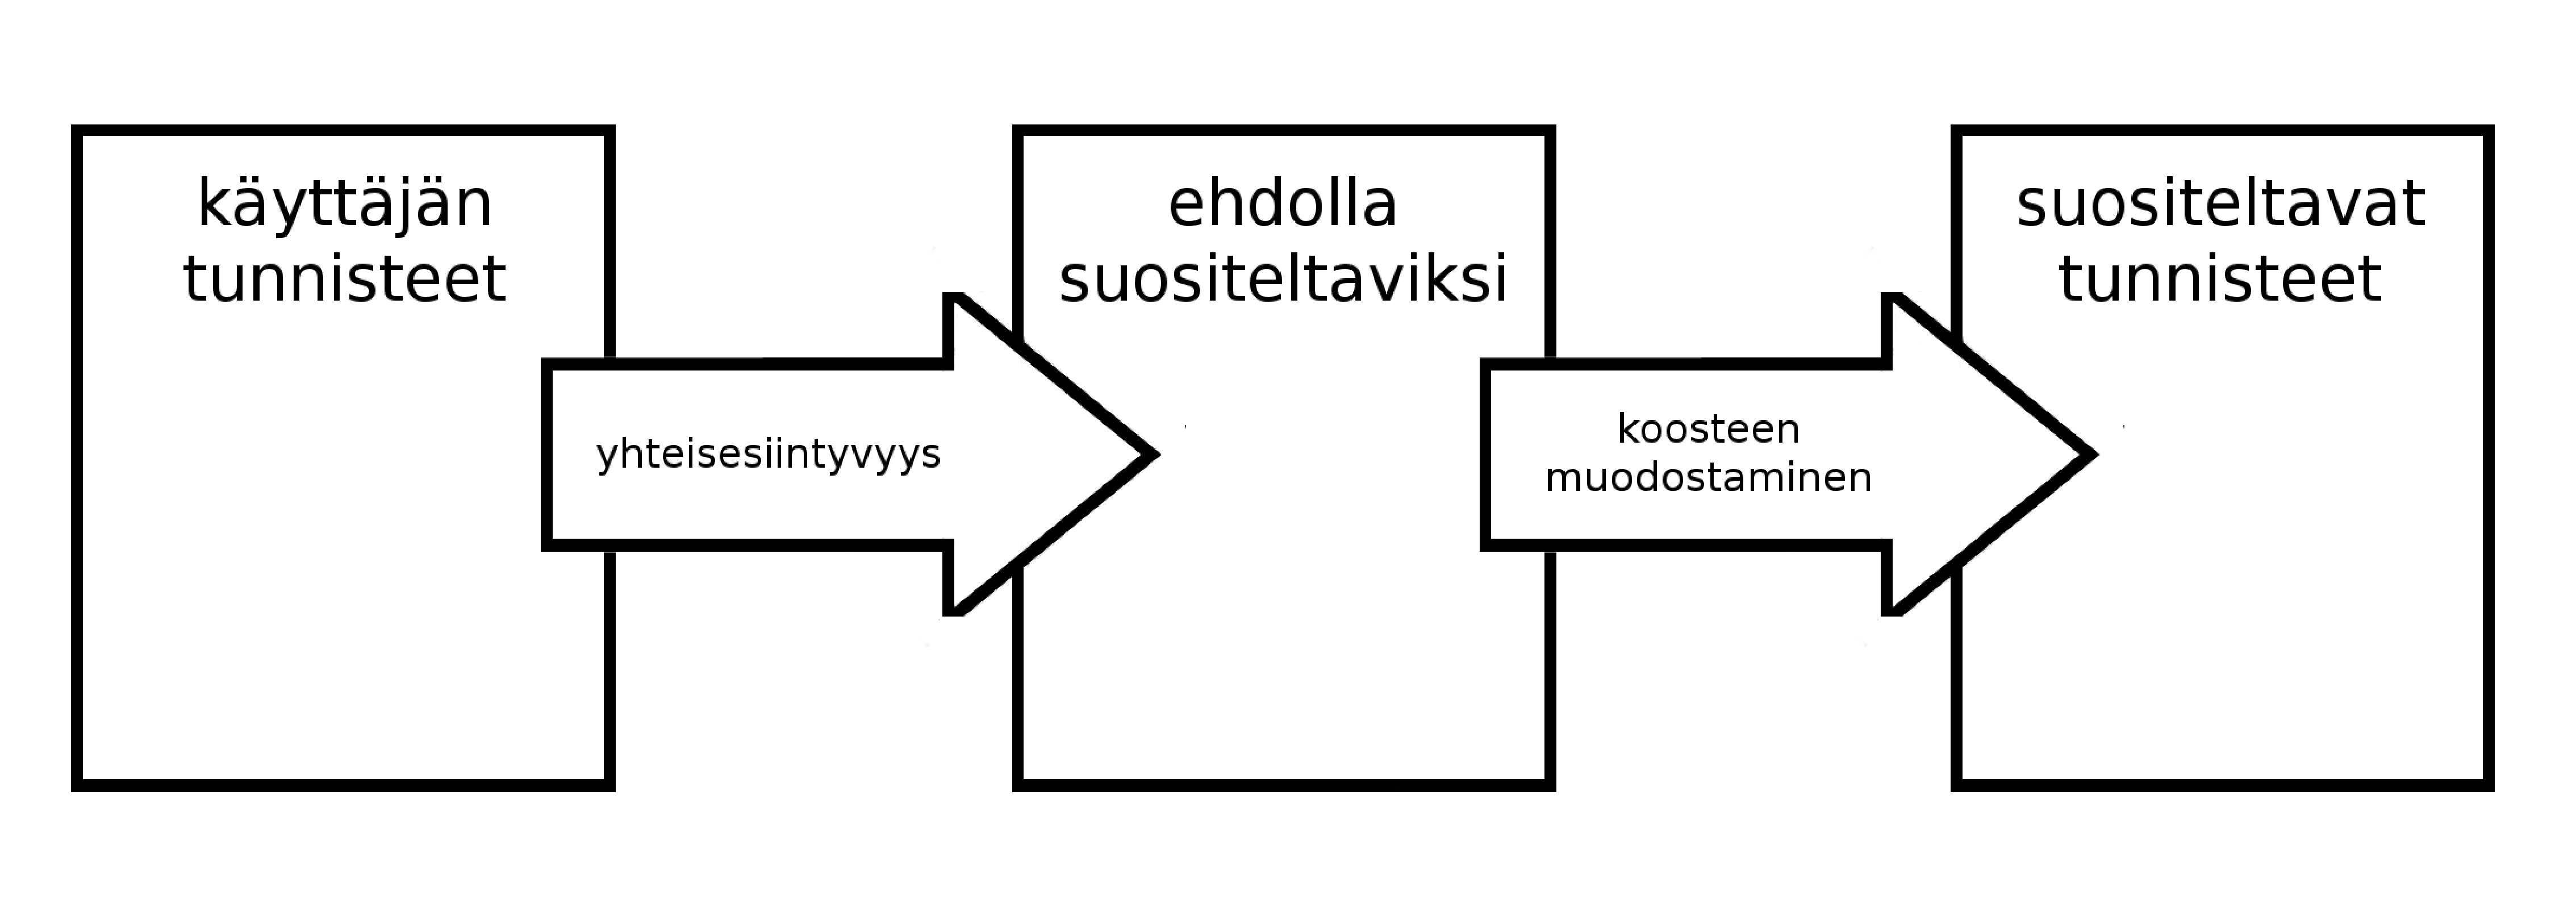
\includegraphics[width = 420pt]{tunnisteidensuosittelu.eps}\caption{Tunnistesuosituksen muodostaminen.}
\label{tunnisteidensuosittelu}
\end{figure}

Jos käyttäjän määrittelemiä tunnisteita on enemmän kuin yksi, mahdollisia suositeltavia tunnisteita on paljon. Tällöin muodostetaan tunnistekooste ja lyhennetään suositeltavien tunnisteiden listaa. Kuvasta \ref{tunnisteidensuosittelu} nähdään tunnistekooste-askeleen sijainti suositteluprosessissa.
Esitellään esimerkiksi summaukseen perustuva tunnistekoosteen muodostaminen. Määritellään kolme tunnisteryhmää seuraavasti:
\begin{enumerate}
\item Käyttäjän määrittelemät tunnisteet $U$.

\item Ehdolla olevat tunnisteet $C_{u}$, jossa $C_{u}$ on järjestetty lista $m$:stä useimmin tunnisteen $u$ kanssa yhteisesiintyvästä tunnisteesta, kun $u \in U$.

\item Suositeltavat tunnisteet $R$, jossa $R$ on järjestetty lista $n$:stä suositteluun parhaiten soveltuvasta tunnisteesta.
\end{enumerate}

Tunnistekooste otetaan kaikkien ehdolla olevien tunnisteiden joukosta $C = \cup_{u\in U}C_u$ ja tulokseksi saadaan lopullinen lista suositeltavista tunnisteista $R$. Summaukseen perustuvassa koosteenmuodostuksessa käytämme $m$:ää useimmin yhteisesiintyvää tunnistetta. Otetaan kaikkien ehdolla olevien tunnisteiden joukosta $C$ yhdiste ja lasketaan yhteen tunnisteiden yhteisesiintymisarvot. Lasketaan ehdolla olevan tunnisteen $c \in C$ arvosana (score)
\begin{displaymath}
score(c) := \sum_{u\in U}1_{c\in C_u}(P(c|u)),
\end{displaymath}
mukaisesti, jossa $1_{c\in C_u}$ saa arvon 1 jos $c\in C_u$ ja arvon 0 muuten. Funktio $P(c|u)$ laskee epäsymmetrisen yhteisesiintymisen kuten aiemmin esitellyssä epäsymmetrisen normalisoinnin funktiossa.

\begin{figure}[]
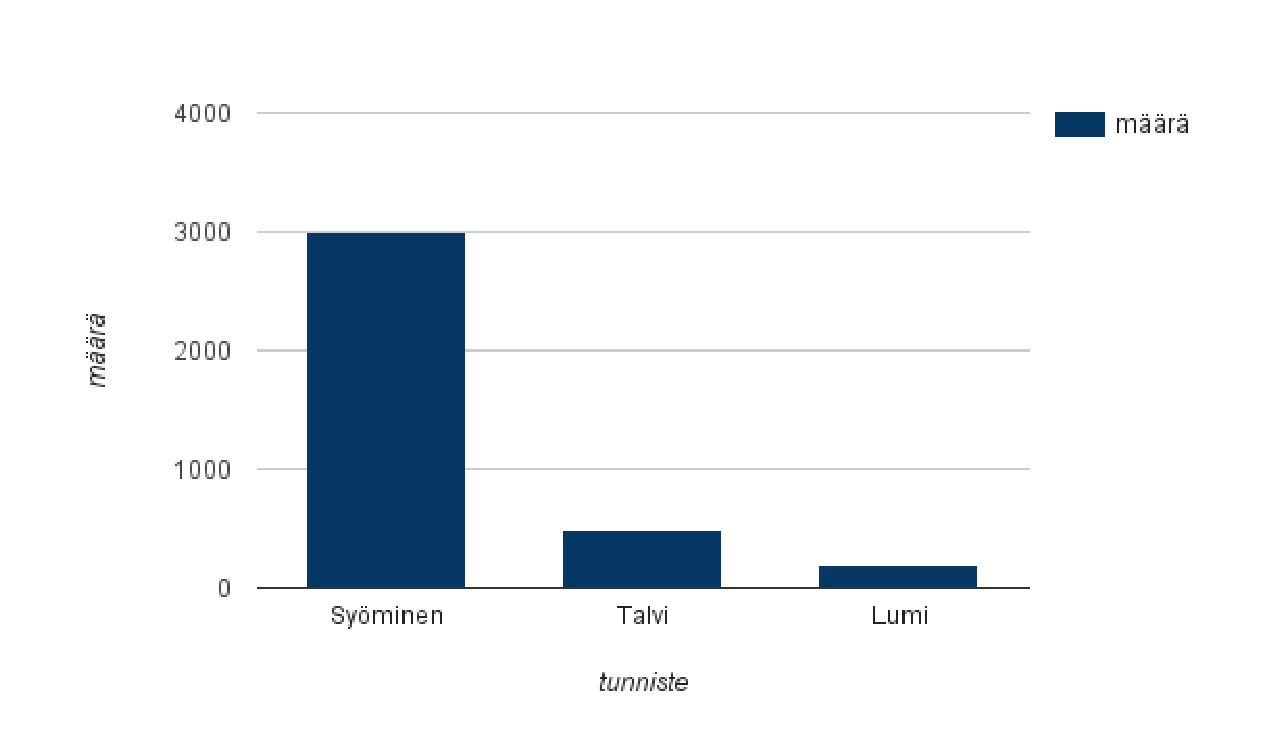
\includegraphics[width = 390pt]{tunnisteet.eps}\caption{Esimerkin tunnisteiden jakautuminen kuvitteellisessa datassa.}
\label{esimerkkitunnisteet}
\end{figure}

Havainnollistetaan seuraavaksi tunnisteiden suosittelua esimerkillä. Tarkastellaan kolmea eri tunnistetta: \textit{Talvi} (500), \textit{Lumi} (200) ja \textit{Syöminen} (3000). Kuvasta \ref{esimerkkitunnisteet} nähdään näiden tunnisteiden esiintymismäärät suhteessa toisiinsa. Tarkastellaan tilannetta jossa käyttäjä merkitsee kuvansa tunnisteella \textit{Talvi}.
\begin{figure}[h]
\centerline{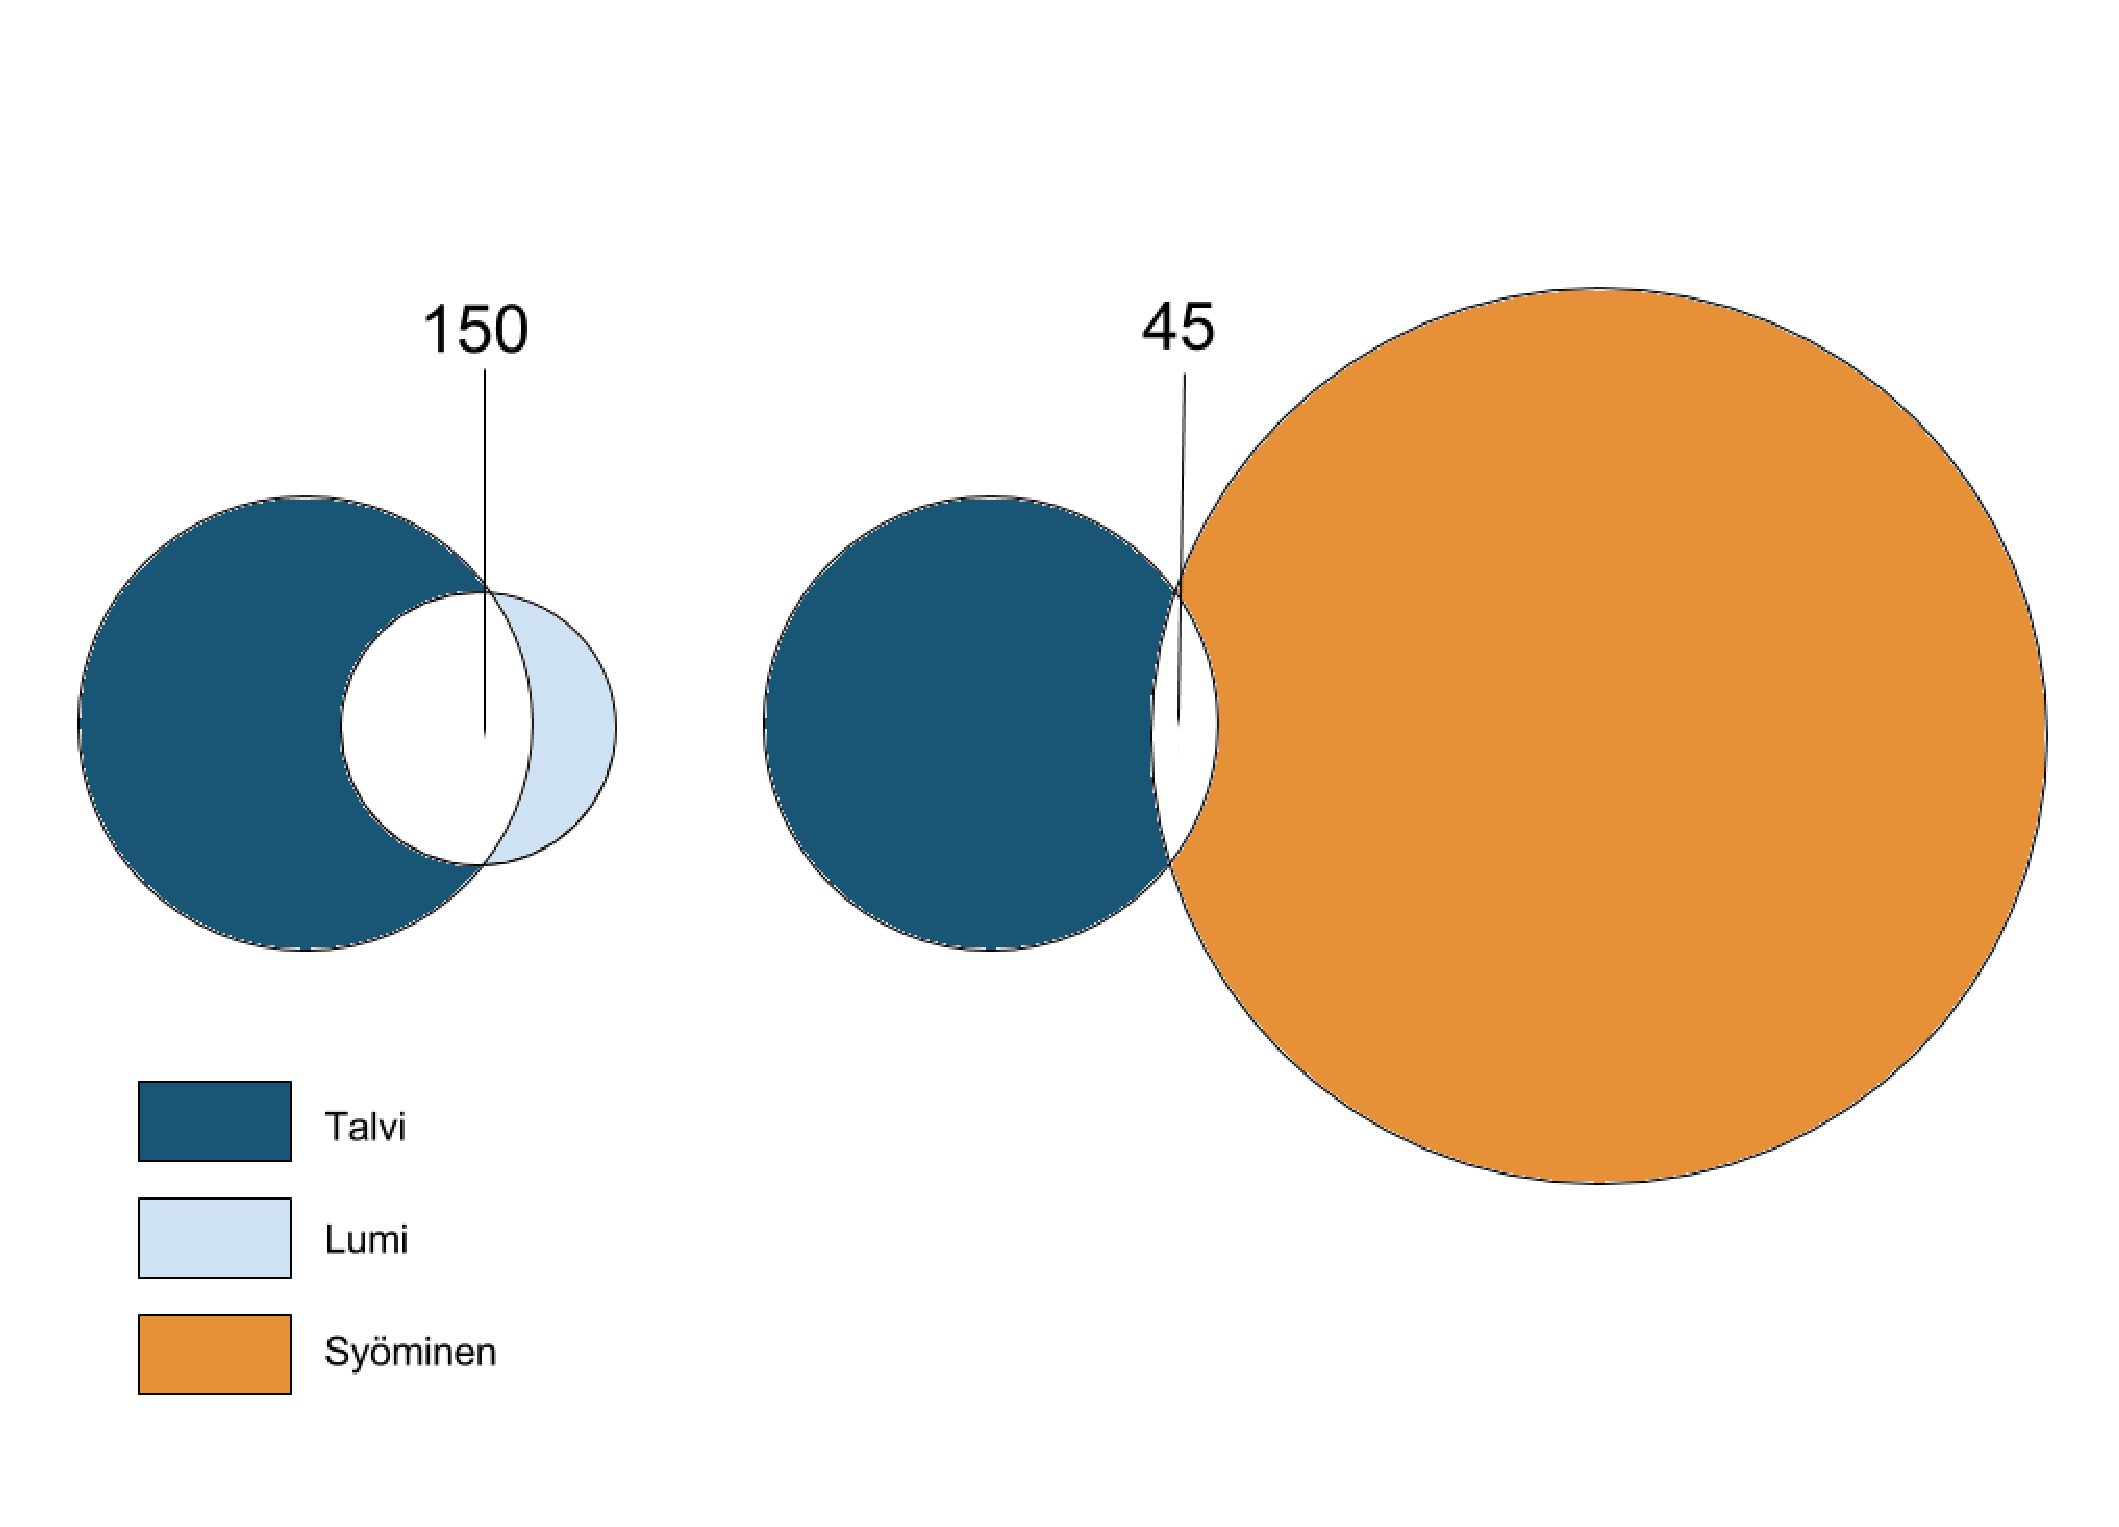
\includegraphics[width = 360pt]{uudetvennit.eps}}\caption{Tarkasteltavien tunnisteiden yhteisesiintyminen.}
\label{vennit}
\end{figure}
Oletetaan, että tunnisteet \textit{Talvi} ja \textit{Lumi} esiintyvät muissa kuvissa yhdessä 150 kertaa ja tunnisteet \textit{Talvi} ja \textit{Syöminen} 45. Tätä tunnisteiden yhteisesiintyvyyttä havainnollistetaan kuvassa \ref{vennit}. Vertaillaan ensin tunnisteiden \textit{Talvi} ja \textit{Lumi} yhteisesiintyvyyttä kaavalla 
\begin{displaymath} 
P (Lumi | Talvi):= \frac{|K(Talvi) \cap K(Lumi)|} {|K(Talvi)|}
\end{displaymath}
josta saadaan luku 0,3.
Kun tehdään sama tunnisteille \textit{Talvi} ja \textit{Syöminen} niin saadaan luku 0,09. 

Tunniste \textit{Lumi} sai korkeamman arvosanan, joten suosittelemme sitä käyttäjälle mieluummin kuin tunnistetta \textit{Syöminen}. Lumi vaikuttaa luontevammalta parilta talvelle kuin syöminen, joten tunnistesuosituksen voidaan sanoa olevan hyödyllinen. Oikeassa tapauksessa yhteisesiintyviä tunnisteita käyttäjän antamalle tunnisteelle olisi paljon enemmän kuin kaksi ja suositeltavien tunnisteiden listakin pitenisi.

Realistisemmassa esimerkissä tulisi olla kriittinen sen suhteen, minkälaiset tunnisteet saavat korkeimman arvosanan. Ensimmäisenä listassa on nimittäin usein niin yleisluontoisia tunnisteita, etteivät ne tarjoa tarpeeksi kuvaavaa informaatiota käsiteltävästä kuvasta \cite{Sigurbjornsson:2008:FTR:1367497.1367542}. Kuten jo kappaleen alussa mainittiin, tällaisia kaikkein yleisimmin käytettyjä tunnisteita ei kannata suositella käyttäjille. Ongelman ratkaisuksi tehdään askel nimeltä kuvailevuuden edistäminen (descriptiveness-promotion) ja alennetaan todella usein esiintyvien tunnisteiden arvosanaa funktiolla
\begin{displaymath}
kuvailevuus(c) := \frac{k_d}{k_d + (|k_d -log(f_c)|)}
\end{displaymath}
jossa $f_c$ on tunnisteen $c$ esiintymistiheisyys aineistossa ja $k_d$ on parametri, joka opitaan datasta. Artikkelissa parametrin $k_d$ oppimiseen käytettiin 131 kuvan joukkoa.

Tarkasteltavassa artikkelissa evaluoitiin kaikkia edellä esiteltyjä funktioita suurilla kuva- ja tunnistejoukoilla. Lisäksi käytettiin toistakin koosteenmuodostusalgoritmia ja esiteltiin kolme suositteluja edelleen parantavaa askelta, joita emme tässä käsitelleet. Ryhmän tekemän evaluoinnin lopuksi todettiin edellä esitellyn suosittelustrategian tuottavan hyödyllisiä tunnistesuosituksia realistisellakin testidatalla~\cite{Sigurbjornsson:2008:FTR:1367497.1367542}.



\section{Yhteistoiminnallisen suodattamisen järjestelmät}
\subsection{Yleisesti}
\begin{figure}[]
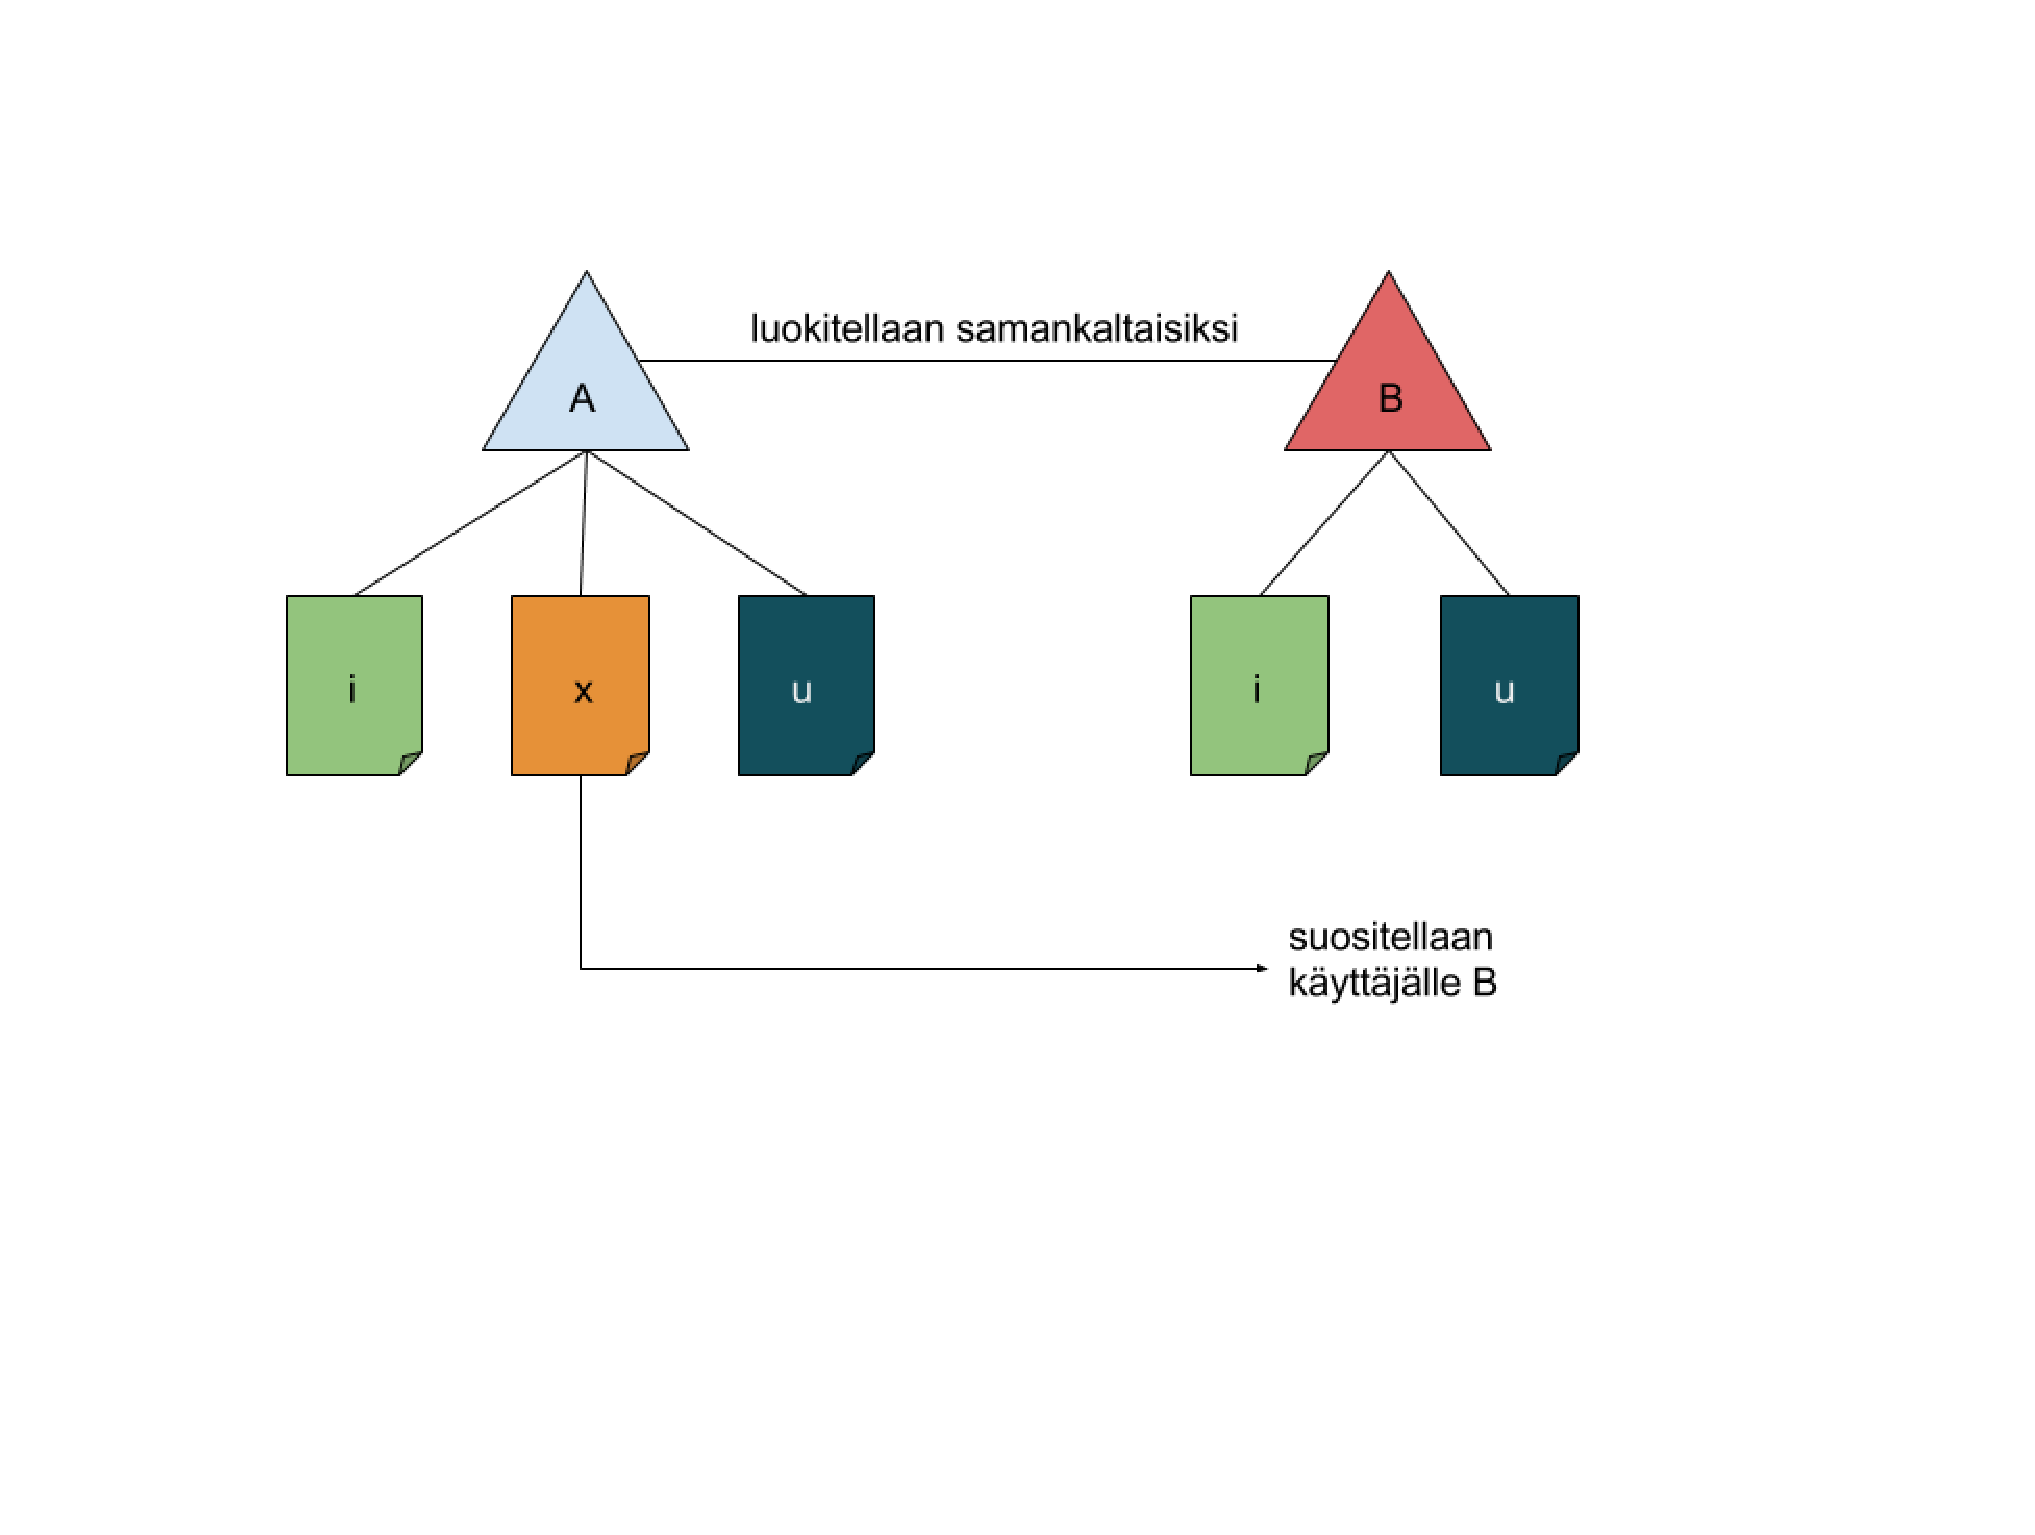
\includegraphics[width = 400pt]{yhteistoiminnallinen.eps}\caption{Havainnollistus yhteistoiminnalliseen suodattamiseen perustuvan suosittelujärjestelmän perusperiaatteesta.}
\label{yhteistoiminnallinen}
\end{figure}
        Yhteistoiminnalliseen suodattamiseen perustuvissa suosittelujärjestelmissä otetaan yksittäisen käyttäjän ja tuotteiden sijasta huomioon kaikkien käyttäjien väliset riippuvuudet. Suositusjärjestelmä vertaa käyttäjästä kerättyjä tietoja muiden käyttäjien tietoihin ja luokittelee käyttäjät samanlaisten mieltymysten perusteella pienemmiksi ryhmiksi. Jos joku tällaisen ryhmän jäsenistä on pitänyt jostakin tietystä tuotteesta, suositellaan tuotetta muillekin ryhmän jäsenille.
        
Kuvassa \ref{yhteistoiminnallinen} on esitelty tällaisen järjestelmän periaate hyvin yleisellä tasolla. Käyttäjät $A$ ja $B$ ovat arvostelleet tuotteet $i$ ja $u$ samalla tavalla siten, että kumpikin pitää näistä tuotteista. Lisäksi käyttäjä $A$ on arvostellut tuotteen $x$ ja osoittanut pitävänsä siitä. Tämän perusteella suositellaan tuotetta $x$ käyttäjälle $B$, jolla ei vielä ole arvostelua kyseisestä tuotteesta.
        
         Automaattisen yhteistoiminnallisen suodattamisen (ACF) järjestelmiä väitetään perinteisiä sisältöpohjaisia tehokkaammaksi, sillä tuotteiden suodattaminen pohjautuu koneanalyysin sijasta käyttäjäyhteisön relaatioihin \cite{Herlocker:2000:ECF:358916.358995}. ACF-järjestelmät toimivat hyvin kaikenlaisen tiedon arvioinnissa, sellaisenkin, jota koneen on vaikea arvioita, kuten ihmisten makutottumukset tai laatuvaatimukset. ACF-järjestelmät eivät kuitenkaan ole syrjäyttäneet sisältöpohjaisia järjestelmiä, vaan niitä käytetään usein rinnakkain \cite{Burke:2002:HRS:586321.586352}.
         
         Yhteistoiminnallisen suodattamisen järjestelmät voidaan jakaa vielä kahteen alatyyppiin: muistipohjaisiin ja mallipohjaisiin \cite{Das:2007:GNP:1242572.1242610}. Muistipohjaiset algoritmit tekevät ennusteita suoraviivaisesti käyttäjien arvosteluhistorioiden perusteella laskemalla eri käyttäjien tai tuotteiden samankaltaisuuksia. Yleisesti käytettäviä samankaltaisuuden mittaustapoja ovat Pearsonin korrelaatiokerroin ja kosinisamankaltaisuus (cosine similarity) arvosteluista muodostettujen vektoreiden välillä.
         
Mallipohjaiset algoritmit käyttävät historioita käyttäjien mallintamiseen ja ennustavat näillä malleilla tulevia arvosteluja kohteille, joita käyttäjät eivät ole vielä nähneet. Mallipohjaisia menetelmiä ovat esimerkiksi Bayesiläinen klusterointi, piilosemanttinen indeksointi (latent semantic indexing, LSI), todennäköisyyspohjainen piilosemanttinen indeksointi (PLSI) ja Markovin päätösprosessi (Markov Decision process)~\cite{Das:2007:GNP:1242572.1242610}.
        
Yleinen tapa toteuttaa yhteistoiminnallisen suodattamisen suosittelujärjestelmä on käyttää muistipohjaisen ja mallipohjaisen tyypin yhdistelmää~\cite{Burke:2002:HRS:586321.586352}. Seuraavissa kappaleissa on esitelty kaksi eri projektia, jotka käyttivät kumpikin näiden tyyppien yhdistelmää.

\subsection{Netflix Prize -kilpailu}

        Suosittelujärjestelmät nousivat suuremman yleisön puheenaiheeksi digitaalisen elokuvavuokraamo Netflixin vuonna 2006 järjestämän Netflix Prize -kilpailun ansiosta. Kilpailun tarkoituksena oli parantaa Netflixin käyttämää suosittelujärjestelmää ja pienentää annetun testidatan keskineliöpoikkeamaa 10 prosentilla. Testidata koostui yli 100 miljoonasta elokuva-arvostelusta noin 480 000 käyttäjältä 17 770 eri elokuvasta. Bell ja Koren käsittelevät artikkelissaan~\cite{Bell:2007:LNP:1345448.1345465} tässä kilpailussa vuoden sisällä parhaiten pärjänneen joukkueen suosittelujärjestelmämallia, joka saavutti 8,43 \%:n parannuksen.
        
        Huomattavaa joukkueen käyttämässä mallissa oli se, että se käytti kahden tärkeimmän yhteistoiminnallisen suodattamisen mallityypin yhdistelmää. Kummassakin mallissa on omat puutteensa, mutta yhdessä ne tuottivat hyviä tuloksia. Kappaleessa 3.1 esitellyn jaon mukaan toinen käytetyistä menetelmistä voidaan luokitella muistipohjaisiin ja toinen mallipohjaisiin algoritmeihin.
        
        Muistipohjaisena algoritmina toimii naapurustomalli (Neighborhood model, k-NN), joka on hyvä havaitsemaan paikallisia riippuvuuksia. Mallilla tarkastellaan kunkin alkion k:ta lähintä naapuria ja luokitellaan käsiteltävä alkio siihen ryhmään, jonka jäseniä on tarkasteltavissa naapureissa eniten. Kuvassa \ref{knn} on havainnollistettu naapurustomallin toimintaa. Mallilla koko tarkasteltava joukko saadaan jaettua pienempiin ryhmiin.
        
\begin{figure}[]
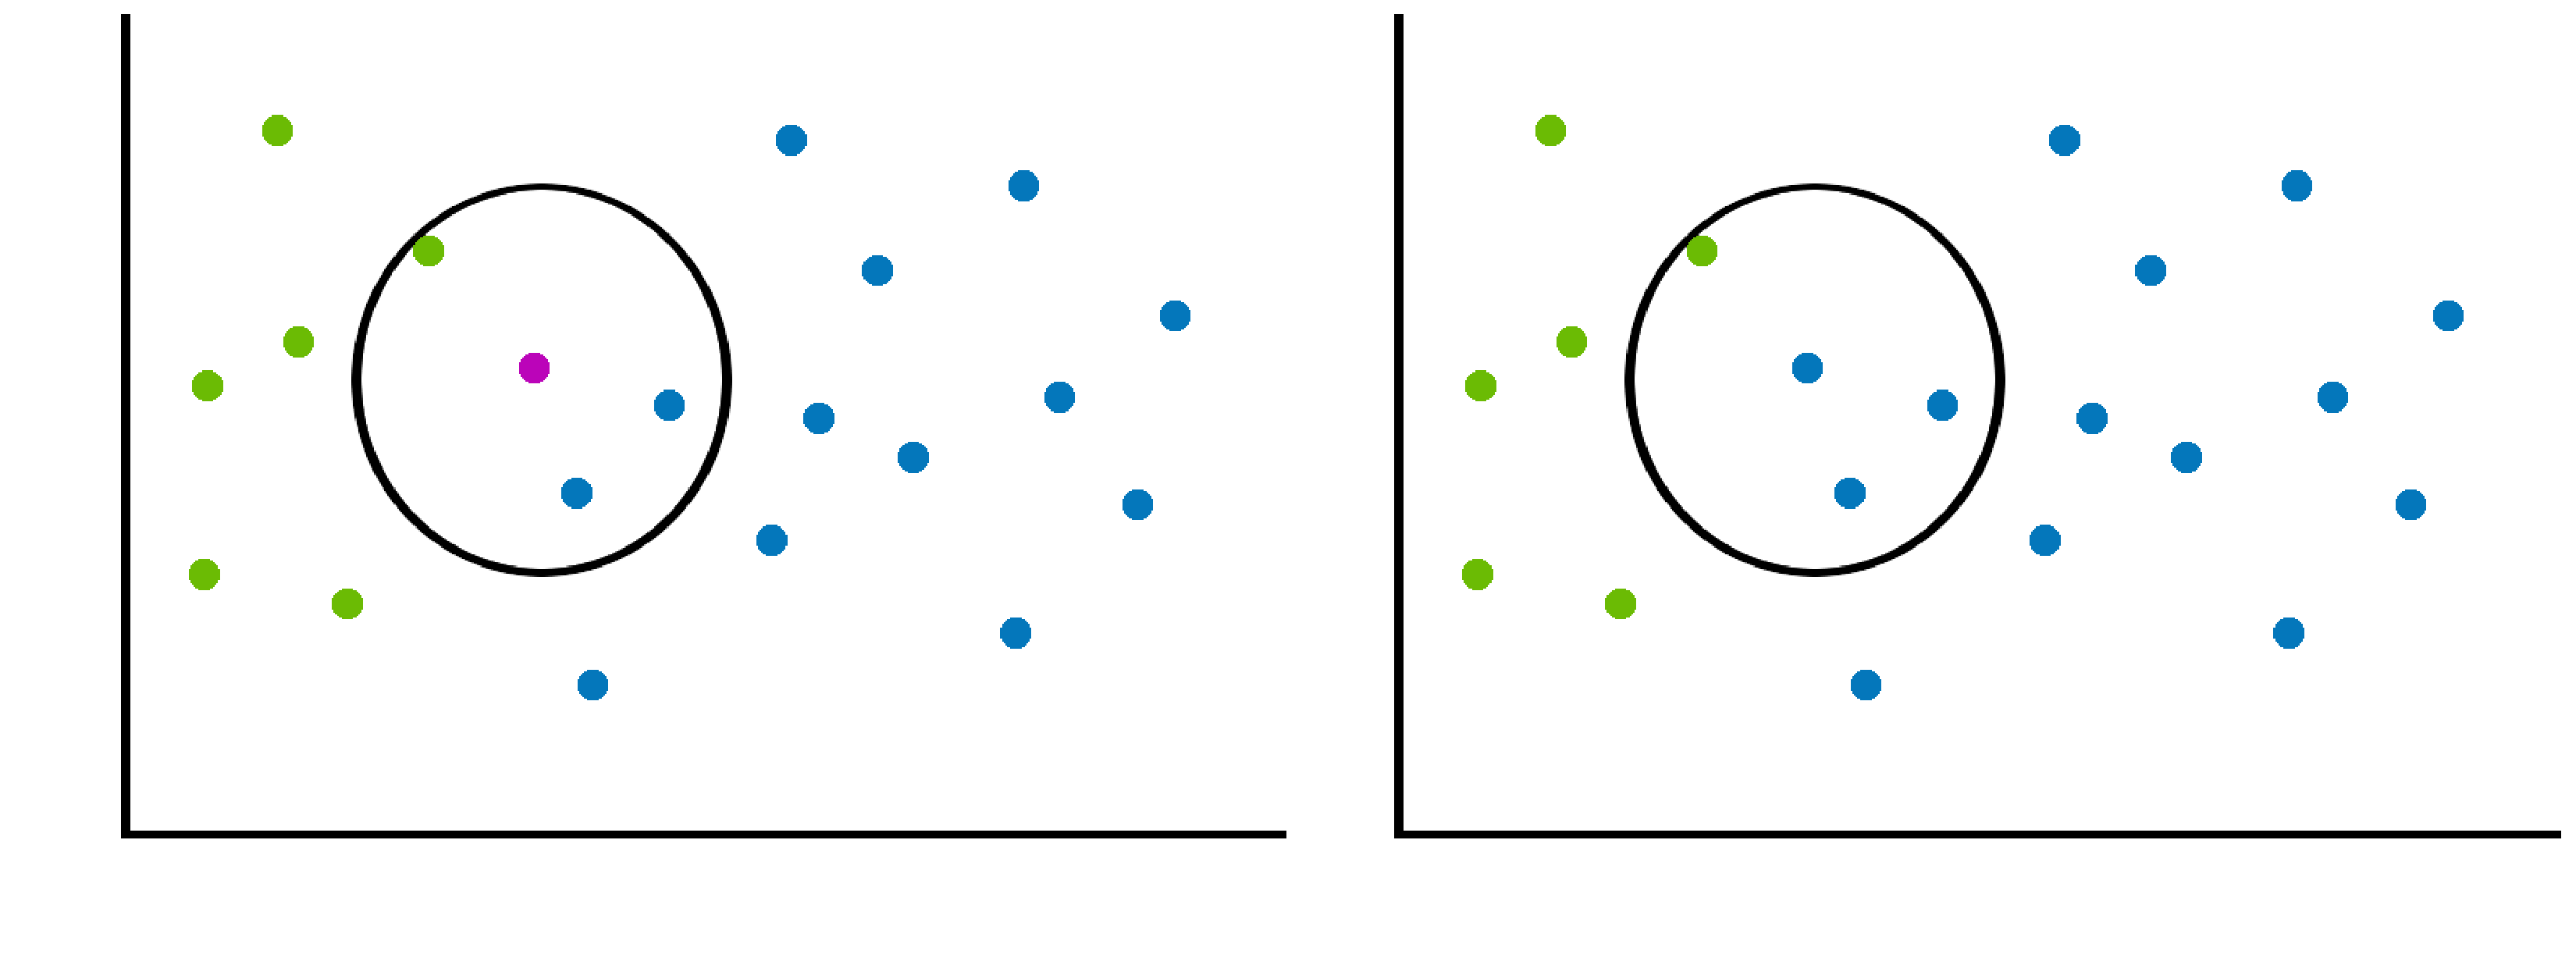
\includegraphics[width = 370pt]{knnkumpikin.eps}\caption{Naapurustomallin (k-NN) perusperiaate. Valitaan violetin yksilön k lähintä naapuria (tässä k = 3). Koska näissä naapureissa on enemmän sinisiä naapureita, luokitellaan violetti sinisten joukkoon.}
\label{knn}
\end{figure} 
 
Joukkueen käyttämässä naapurustomallissa elokuvat jaotellaan pareihin, jotka on arvosteltu pääsääntöisesti samalla tavalla. Näiden parien avulla pyritään ennustamaan käyttäjän mielipide elokuvasta, jota hän ei ole arvostellut. Naapurustomalli ottaa huomioon vain osan käyttäjän arvosteluista eikä siis havaitse niissä piileviä heikkoja signaaleja. 

	Piilomuuttujamallit tulevat apuun siinä, missä naapurustomallissa on puutteita. Kun naapurustomalli havaitsee vain samankaltaisten elokuvien suhteet, hahmottaa piilomuuttujamalli elokuvien väliset riippuvuudet kattavammin. Se pystyy esimerkiksi havaitsemaan saman lajityypin elokuvien olevan samankaltaisia keskenään. Toisin kuin naapurustomallit, se ei kuitenkaan huomioi pieniä, keskenään samankaltaisista elokuvista muodostuvia ryhmiä. Malli ei esimerkiksi pysty suosittelemaan trilogian ensimmäisen osan katsoneelle käyttäjälle sarjan toista osaa. Joukkueen käyttämän piilomuuttujamallin toiminta perustuu käyttäjästä ja elokuvasta muodostettaviin vektoreihin, joiden avulla saadaan ennuste käyttäjän arviolle elokuvasta.
        
	Koren esittelee käytettyjen mallien teknistä puolta tarkemmin omassa artikkelissaan \cite{Koren:2008:FMN:1401890.1401944}. Tutustumme kahdesta esitellystä mallista lähemmin naapurustomalliin. Perinteistä naapurustomallia ei käytetty sellaisenaan, vaan sitä paranneltiin käyttötarkoitukseen sopivaksi. Pohjalla ollut, yleisesti käytössä oleva korrelaatioihin perustuva naapurustomalli,
\begin{displaymath}
\hat{r}_{ui} = b_{ui} + \frac{\sum_{j\in S^{k}(i;u)} s_{ij}(r_{uj}-b_{uj})}{\sum_{j \in S^{k} (i;u)}s_{ij} }
\end{displaymath}         
antaa käyttäjän $u$ ennustetun arvion $r_{u_{i}}$ tuotteelle $i$. Mallissa
\begin{enumerate}
\item Ennuste $r_{u_{i}}$ otetaan naapurituotteiden arvosteluiden painotettuna keskiarvona.
\item Funktio $b_{ui} = \mu + b_u + b_i$ antaa pohja-arvion (baseline estimate) jossa $b_u$ on käyttäjän $u$ havaittu poikkeama keskiarvosta ja $b_i$ vastaavasti tuotteen $i$ havaittu poikkeama keskiarvosta. Parametri $\mu$ on keskimääräinen arvosana tuotteen arviolle.
\item Joukko $S^k (i;u)$ sisältää $k$ käyttäjän $u$ arvostelemaa kaikkein samankaltaisinta tuotetta tuotteen $i$ kanssa.
\item Funktio $s_{ij}$ mittaa tuotteiden samankaltaisuutta $s_{ij} \stackrel{def}{=} \frac{n_{ij}}{n_{ij} + \lambda_2} p_{ij}$, jossa $n_{ij}$ on niiden käyttäjien lukumäärä, jotka arvostelivat tuotteet $i$ ja $j$. Tyypillinen arvo parametrille $\lambda_2$ on 100. Samankaltaisuuden mittaamisen pohjana on Pearsonin korrelaatiokerroin $p_{ij}$.
\end{enumerate} 

Tällaisenaan käytettynä malli ei kuitenkaan ole täysin ongelmaton. Ryhmä näki suurimpana ongelmana sen, että metodin toiminnalle ei ole olemassa formaalia perustelua. Lisäksi samankaltaisuusmittauksen huomautettiin keskittyvän vain kahden tuotteen relaatioihin jättämällä näin huomiotta suhteet muuhun naapuristoon. Kolmanneksi todettiin, että interpolaatiopainojen summautuessa yhteen on mallin pakko nojautua naapureihin sellaisissakin tapauksissa, kun naapurustotietoa ei löydy, eli käyttäjä $u$ ei ole arvioinut tuotteen $i$ kanssa samanlaisia tuotteita. Tällöin olisi järkevämpää katsoa pohja-arviota naapuruuksien sijaan \cite{Koren:2008:FMN:1401890.1401944}.
Ongelmat ratkaistiin päivitetyllä mallilla
\begin{displaymath}
\hat{r}_{ui} = b_{ui} + \sum_{j\in{S^{k}} (i;u)}\theta^{u}_{ij}(r_{uj}-b_{uj})
\end{displaymath}
jossa annetulle joukolle naapureita $S^{k}(i;u)$ lasketaan interpolaatiopainot $\theta^{u}_{ij} \in S^{k}(i;u)$. Uudistettu malli tuotti testeissä huomattavasti parempia tuloksia kuin alkuperäinen naapurustomalli, kun $k$:n arvo oli vähintään 500 \cite{Koren:2008:FMN:1401890.1401944}.
                
        Joukkue huomasi olevan oleellista katsoa dataa muutenkin kuin arvostelujen sisältöjen osalta. Laajemman kuvan saamiseksi joukkue keskittyi myös siihen, minkä tyyppisiä elokuvia käyttäjä ylipäätään vaivautuu arvostelemaan. Se, minkä elokuvan käyttäjä kokee arvostelun arvoiseksi, opettaa paljon käyttäjän ajattelumaailmasta. Huonoimmalla arvosanalla arvosteltu elokuva tarjoaa enemmän tietoa kuin arvostelematon, mitäänsanomaton elokuva. Jotkut mallit ottivat huomioon myös muun muassa arvostelujen määrän, keskiarvon ja päivämäärät.
        
Haasteetta projektille toi ihmisten elokuvamaun mallintamisen vaikeus. Mallinnuksessa tulisi ottaa huomioon muun muassa sellaisia piirteitä kun tietynlainen tunnelma, äänimaailma tai dialogin laadukkuus ja päätellä niistä käyttäjän elokuvamakua. Tällaisten ominaisuuksien huomioon ottaminen on kuitenkin algoritmisesti hyvin vaikeaa, sillä käyttäjien mieltymykset eivät ole aina johdonmukaisia. Käyttäjä voi esimerkiksi antaa yksittäiselle elokuvalle viisi tähteä perusteella "se on niin huono että se on hyvä", vaikka normaalisti antaisi vastaaville elokuville yhden tähden~\cite{Bell:2007:LNP:1345448.1345465}.
        
        Projektia vaikeuttivat myös käyttäjien vähäiset tai hajanaiset arviot testidatassa. Joukkue kehitti sekä naapurustomallia että piilomuuttujamallia tehokkaammaksi ja tarkoitukseen sopivammiksi. Eniten ongelmia tuotti datassa esiintyvä puutteellisuus arvojen osalta. Käytettävät mallit ovat standardimuodoltaan sellaisia, etteivät ne huomioi arvosteluiden vähäisyyttä. Jossakin tapauksessa olisi järkevämpää jättää jokin arvo kokonaan huomiotta kuin vääristää laskentaa puutteellisilla tiedoilla. Tästä aiheutuva ylisovittaminen (over fitting) oli yksi ongelma, jota saatiin vähennettyä parannetuilla malleilla.
        
Artikkelin julkaisemisen jälkeen Netflixin toimintaperiaate on muuttunut elokuvavuokraamosta suoratoistopalveluksi. Tämä vaikuttaa datan muotoon ja käyttäjien käyttäytymiseen. Myös suosittelujärjestelmien toimintaa on siksi muutettu edellä esitellyistä malleista. Artikkelissa ennakoitiin muutosta pohdinnassa, jossa esitettiin parempia suosittelutuloksia saatavan aikaiseksi seuraamalla itse arvostelujen ohella muita tietoja. Tällaisia ovat esimerkiksi käyttäjän selaus- tai hakuhistoria~\cite{Bell:2007:LNP:1345448.1345465}.

\subsection{Uutisartikkelien suosittelu käyttäjille - skaalautuva yhteistoiminnallinen suodattaminen}

Google News on palvelu, joka kokoaa käyttäjilleen uutisartikkeleita monelta eri uutissivustolta ja luokittelee keskenään samanlaiset artikkelit ryhmiin. Käyttäjille tarjotaan suosituksia luettavista artikkeleista heidän lukuhistoriansa perusteella. Das ym. \cite{Das:2007:GNP:1242572.1242610} esittelevät artikkelissaan yhteistoiminnalliseen suodattamiseen perustuvan ratkaisuehdotuksensa suosittelujen tarjoamiseen. Ryhmän päätavoitteenaan oli rakentaa skaalautuva online-suosittelujärjestelmä, jota voitaisiin käyttää suurissa palveluissa kuten Google Newsissä.

Google News -palvelun ominaisuudet loivat haasteita järjestelmän rakentamiselle. Valtava kävijämäärä ja miljoonat uutisartikkelit asettavat vaatimuksen skaalautuvuudelle. Palvelun osiot ovat myös jatkuvassa muutoksen tilassa, kun artikkeleita poistuu ja lisätään muutaman minuutin välein. Toisin kuin monissa muissa staattisissa palveluissa, käytettävä suosittelumalli vanhenee nopeasti eikä korjaannu pienillä muutoksilla. Osioiden jatkuva muutos on merkittävin tekijä, joka erottaa rakennettavan järjestelmän muiden suurien palveluiden suosittelujärjestelmistä \cite{Das:2007:GNP:1242572.1242610}.
\begin{figure}[]
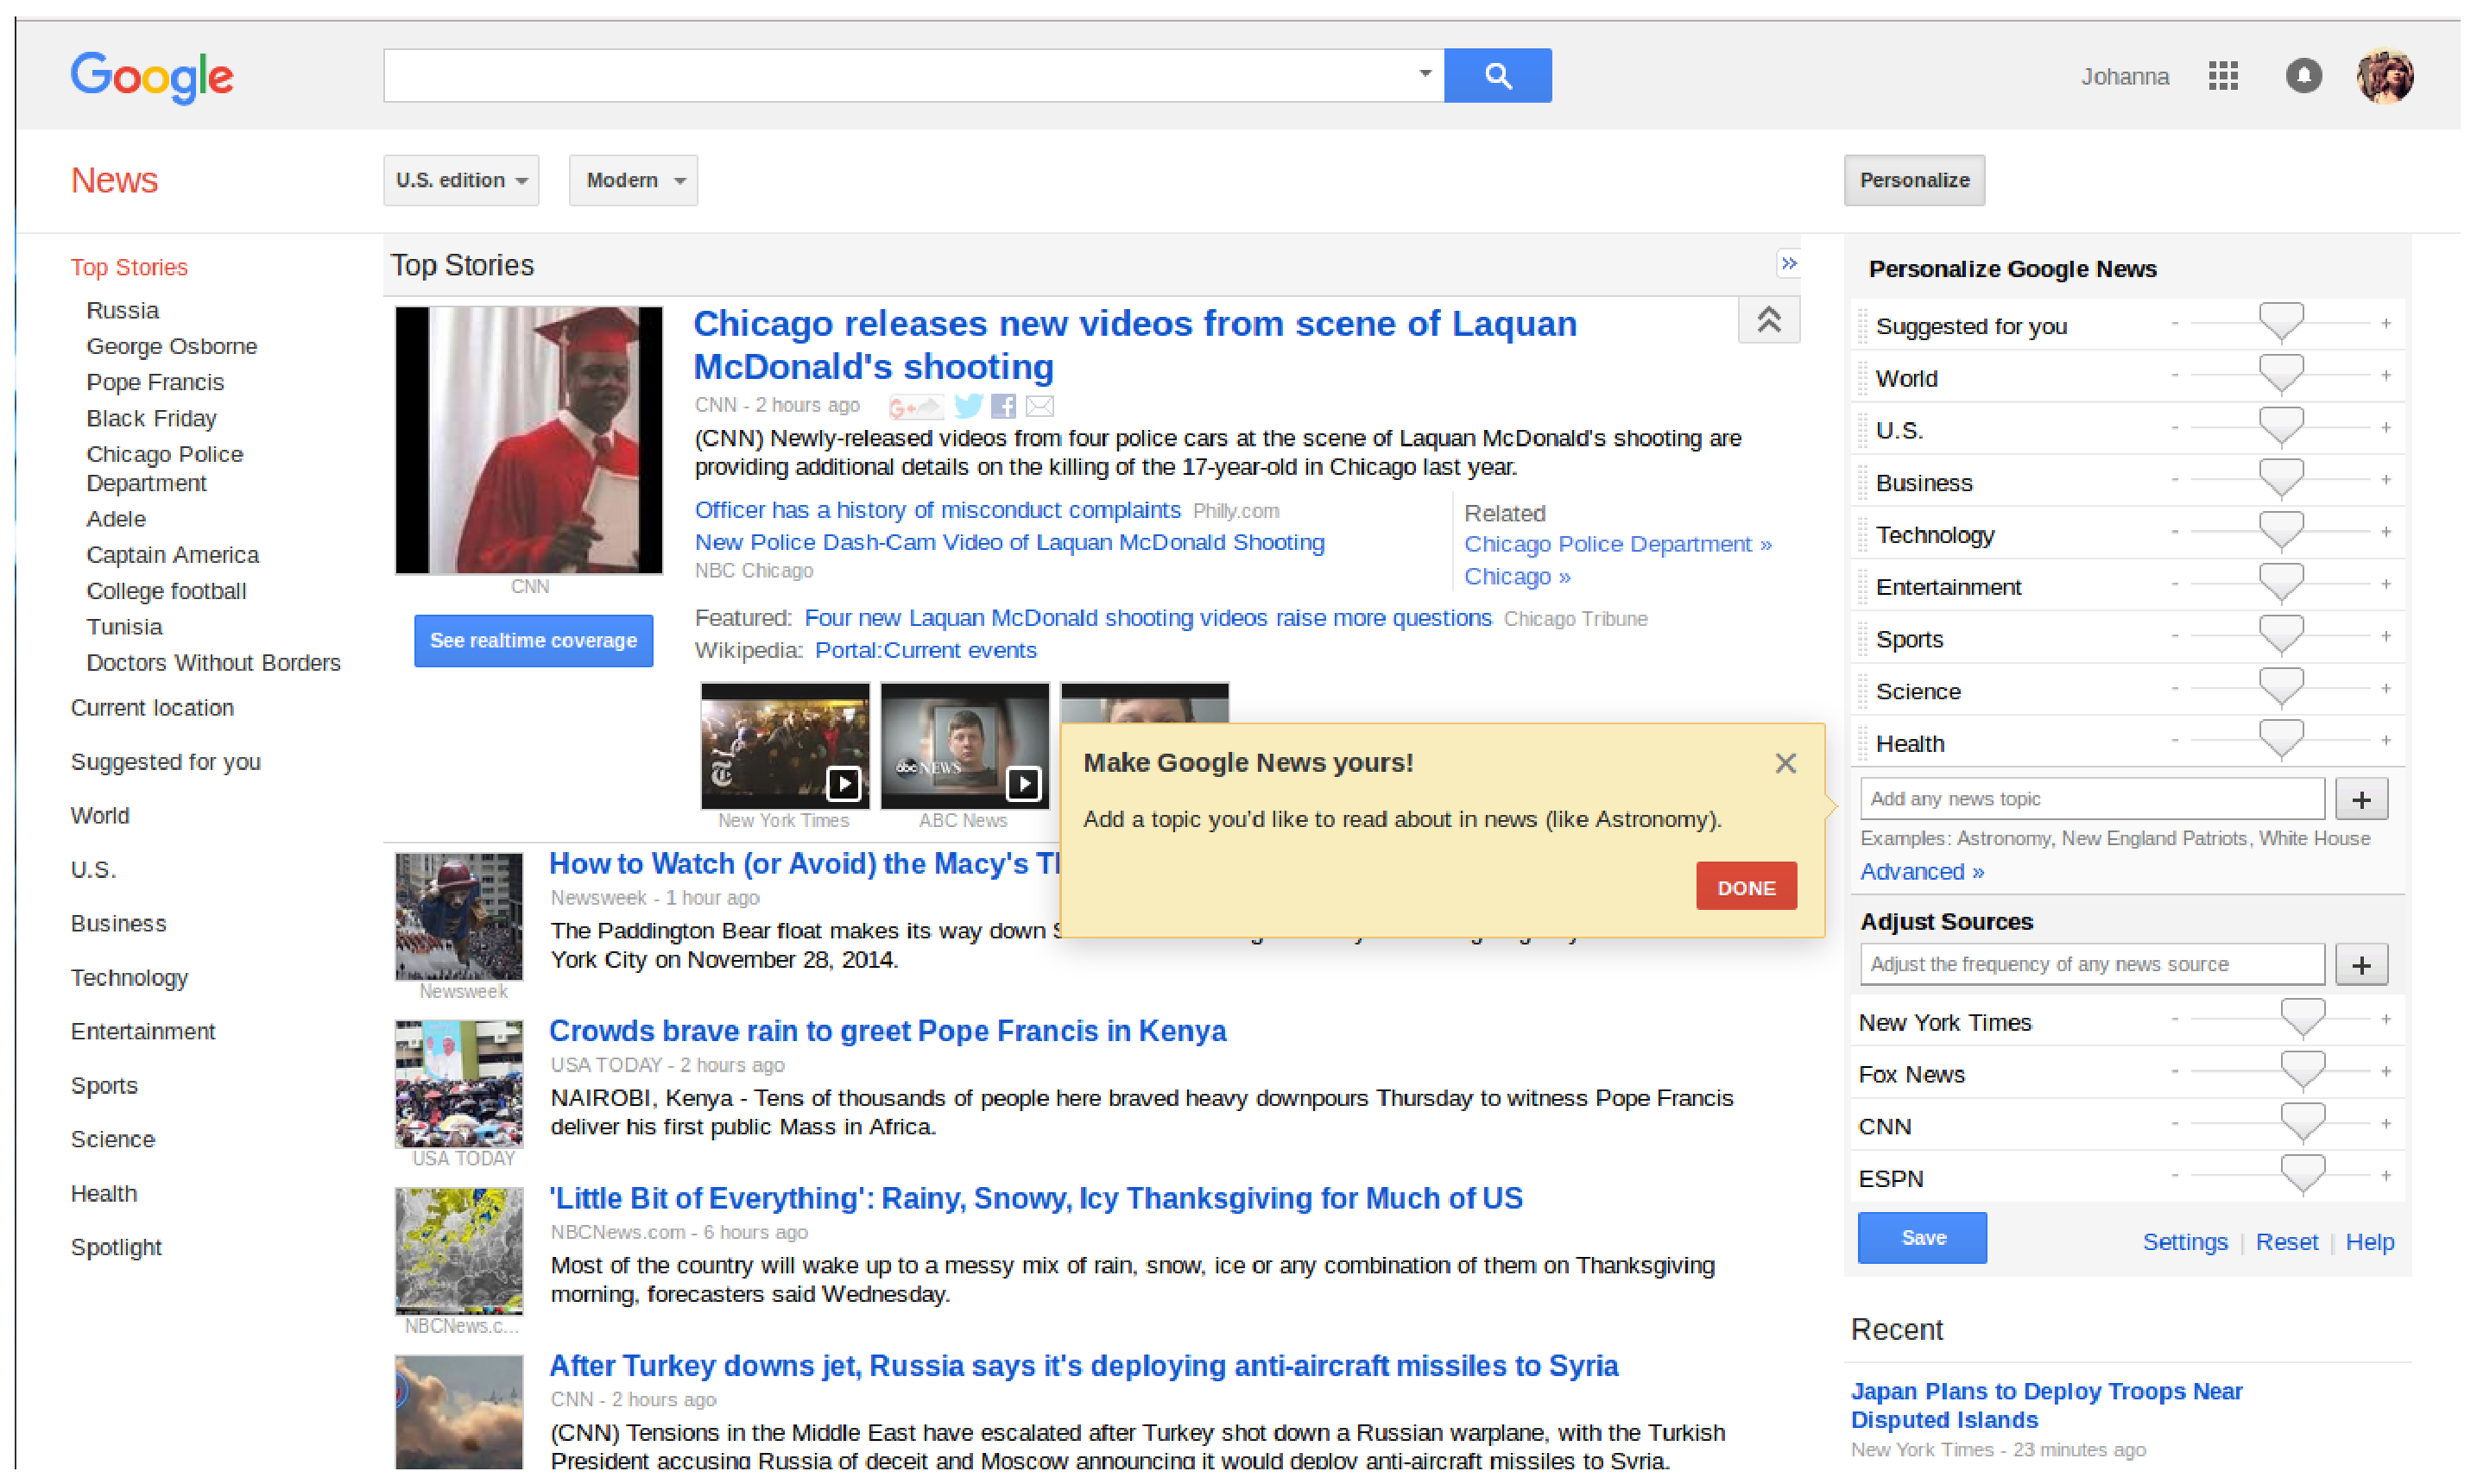
\includegraphics[width = 390pt]{googlenews.eps}\caption{Kuvankaappaus Google Newsistä.}
\label{googlenews}
\end{figure} 

Google News -palvelulla on käyttäjänä sekä rekisteröitymättömiä että rekisteröityneitä käyttäjiä, joista jälkimmäisille tarjotaan enemmän käytettäviä ominaisuuksia. Kuvassa \ref{googlenews} näkyy rekisteröityneen käyttäjän näkymä palvelussa. Käyttäjän niin salliessa Google tallentaa rekisteröityneen käyttäjän uutisartikkeleihin liittyviä aktiviteetteja muiltakin Googlen palveluilta ja tallentaa nämä artikkelit käyttäjän lukuhistoriaan Google News -palvelussa. Esimerkki tällaisesta aktiviteetista voisi olla vaikka uutisartikkelin hakeminen Googlen hakukoneella. Kootun historian pohjalta muodostetaan artikkelisuosituksia, joista kolmea tarjotaan käyttäjän luettavaksi. Artikkelin projektissa keskityttiin suosituksien antamiseen juurikin rekisteröityneille käyttäjille. 

Toisin kuin joissakin suositusjärjestelmiä käyttävissä palveluissa, Google Newsissä tarkasteltavat tuotteet eivät saa suoraa arvosanaa käyttäjältään. Projektissa päätettiinkin käsitellä käyttäjän käyttäytymistä arvioinnin pohjana siten, että klikkaus uutisartikkeliin tulkitaan myönteisenä äänenä artikkelille. Päätöstä perusteltiin sillä, että käyttäjille tarjotaan lyhyt, selkeä kuvaus jokaisesta artikkelista listausnäkymässä. Voidaan siis olettaa, että käyttäjä on todennäköisimmin kiinnostunut artikkelista, jos hän vielä kuvauskappaleen lukemisenkin jälkeen päättää klikata artikkelia. Klikkaukset kuvastavat kuitenkin vain käyttäjien myönteisiä mielipiteitä, eivätkä kerro mitään siitä, mistä käyttäjät eivät pidä \cite{Das:2007:GNP:1242572.1242610}.

Google News -palvelu on yksi maailman suosituimmista uutissivustoista. Tarkasteltavassa projektissa havainnoitiin uutisartikkeleita yhden kuukauden ajalta ja artikkeleita kertyi useita miljoonia. Käyttäjien klikkausaktiivisuus artikkeleihin on hyvin vaihtelevaa ja klikkaushistorioiden koko vaihtelee nollasta satoihin tai jopa tuhansiin.

Google asettaa tarkkoja vaatimuksia palveluidensa vasteajoille myös Google Newsin kohdalla. Esimerkiksi kotisivun näkymä generoidaan tyypillisesti sekunnissa. Tästä sekunnista jää muiden toimintojen jälkeen jäljelle muutama sata millisekuntia suositteluiden muodostamiseen. Tiukat aikavaatimukset olivatkin yksi projektin haasteista.

Kappaleessa 3.1 esiteltiin jako malli- ja muistipohjaisiin yhteistoiminnallisen suodattamisen järjestelmiin. Artikkelissa käsiteltävässä järjestelmässä käytettiin niin sanottua hybridimallia, eli sekoitusta kummankin tyyppisestä järjestelmästä.

Muistipohjaisena algoritmina toimii Covisitation, jota esitellään tarkemmin jäljempänä. Mallipohjaisessa lähestymisessä käytetään kahta klusterointitekniikkaa, algoritmeja PLSI (todennäköisyyspohjainen piilosemanttinen indeksointi) ja MinHash. Kaikki nämä kolme algoritmia asettavat tarkasteltaville uutisartikkeleille arvosanat siten, että paremmat suositukset saavat korkeamman numeerisen arvon. Lopussa kaikki kolme arvosanaa yhdistetään painottaen kaavalla
\begin{displaymath}
\sum_a{w_a r^{(a)}_{s}}
\end{displaymath}
missä $w_a$ on algoritmin $a$ paino ja $r^{(a)}_{s}$ on algoritmin $a$ antama arvosana artikkelille $s$ ja saadaan järjestetty lista artikkeleita. Tästä listasta valitaan K parhaimman arvosanan saanutta artikkelia ja suositellaan niitä käyttäjälle.

Ensimmäisenä esittelemme todennäköisyyspohjaisen klusterointialgortimin MinHash. MinHash jakaa parin käyttäjiä samaan klusteriin sen todennäköisyyden perusteella, jolla käyttäjät ovat äänestäneet eli klikanneet samoja artikkeleita. Jokainen käyttäjä $u \in U$ esitetään tämän klikkaushistoriana $C_u$, eli joukkona artikkeleita, joita kyseinen käyttäjä on klikannut.

Kahden käyttäjän $u_i$ ja $u_j$ samankaltaisuus on mahdollista mitata käyttämällä jo kappaleessa 2.2 esiteltyä Jaccardin kerrointa $S(u_i, u_j) = \frac{|C_{u_{i}} \cap C_{u_{j}}|}{|C_{u_{i}} \cup C_{u_{j}}|}$. Jos haluaisimme tarjota käyttäjälle $u_i$ suosittelua, laskisimme ensin tämän samankaltaisuuden kaikkien muiden käyttäjien $u_j$ kanssa ja suosittelisimme sitten (käyttäjälle $u_i$) muiden käyttäjien $u_j$ äänestämiä artikkeleita, joiden paino on yhtäläinen suureen $S(u_i, u_j)$ kanssa. Tämän tekeminen reaaliajassa ei kuitenkaan ole skaalautuvaa, joten Jaccardin kerroin ei semmoisenaan kelpaa artikkelin projektin käyttöön.

Ongelman ratkaisuna käytetään tiivisteiden muodostamista LSH-tekniikalla (Locality Sensitive Hashing). LSH:n keskeinen ajatus on muodostaa datapisteistä tiiviste useita tiivistefunktioita käyttäen ja päätellä läheiset naapurit kyselypisteen tiivisteen avulla. Jaccardin kertoimen kanssa käytettäväksi soveltuu LSH-tekniikka MinHash. MinHashin perusidea on permutoida satunnainen joukko artikkeleita ($S$) ja laskea jokaiselle käyttäjälle $u_i$ tiivistearvo indeksinään ensimmäinen artikkeli permutaatiossa, joka kuuluu käyttäjän artikkelijoukkoon $C_{u_{i}}$. Todennäköisyys, että kahdella kaikkien $S$:n permutaatioiden joukosta valitulla permutaatiolla on sama tiiviste, on täysin yhtenevä  niiden Jaccardin kerroin -luvun eli samanlaisuuden kanssa. MinHashin jokaisen tiivisteluokan voidaan ajatella vastaavan klusteria. Samaan klusteriin laitetaan kaksi käyttäjää todennäköisyydellä, joka on yhtenevä näiden käyttäjien artikkelijoukkojen samankaltaisuudella $S(u_i, u_j)$.

Toinen esitelty klusterointialgoritmi PLSI mallintaa käyttäjät ($u \in U$) ja artikkelit ($s \in S$) satunnaismuuttujina.
Käyttäjien ja artikkeleiden väliset suhteet opitaan mallintamalla yhteisjakauma käyttäjistä ja artikkeleista sekoitejakaumana (mixture distribution).
Suhdetta merkitään piilomuuttujalla Z, jonka voidaan ajatella kuvastavan käyttäjä- ja artikkeliyhteisöjä siten, että samankaltaiset käyttäjät ovat oma yhteisönsä ja samankaltaiset artikkelit omansa. Malli voidaan kirjoittaa sekoitemallina
\begin{displaymath}
p(s|u;\theta)= \sum_{z \in Z} {p(z|u)}{p(s|z)}
\end{displaymath}
kun $\theta$ on todennäköisyysjakauman parametrit sisältävä vektori.

\begin{figure}[]
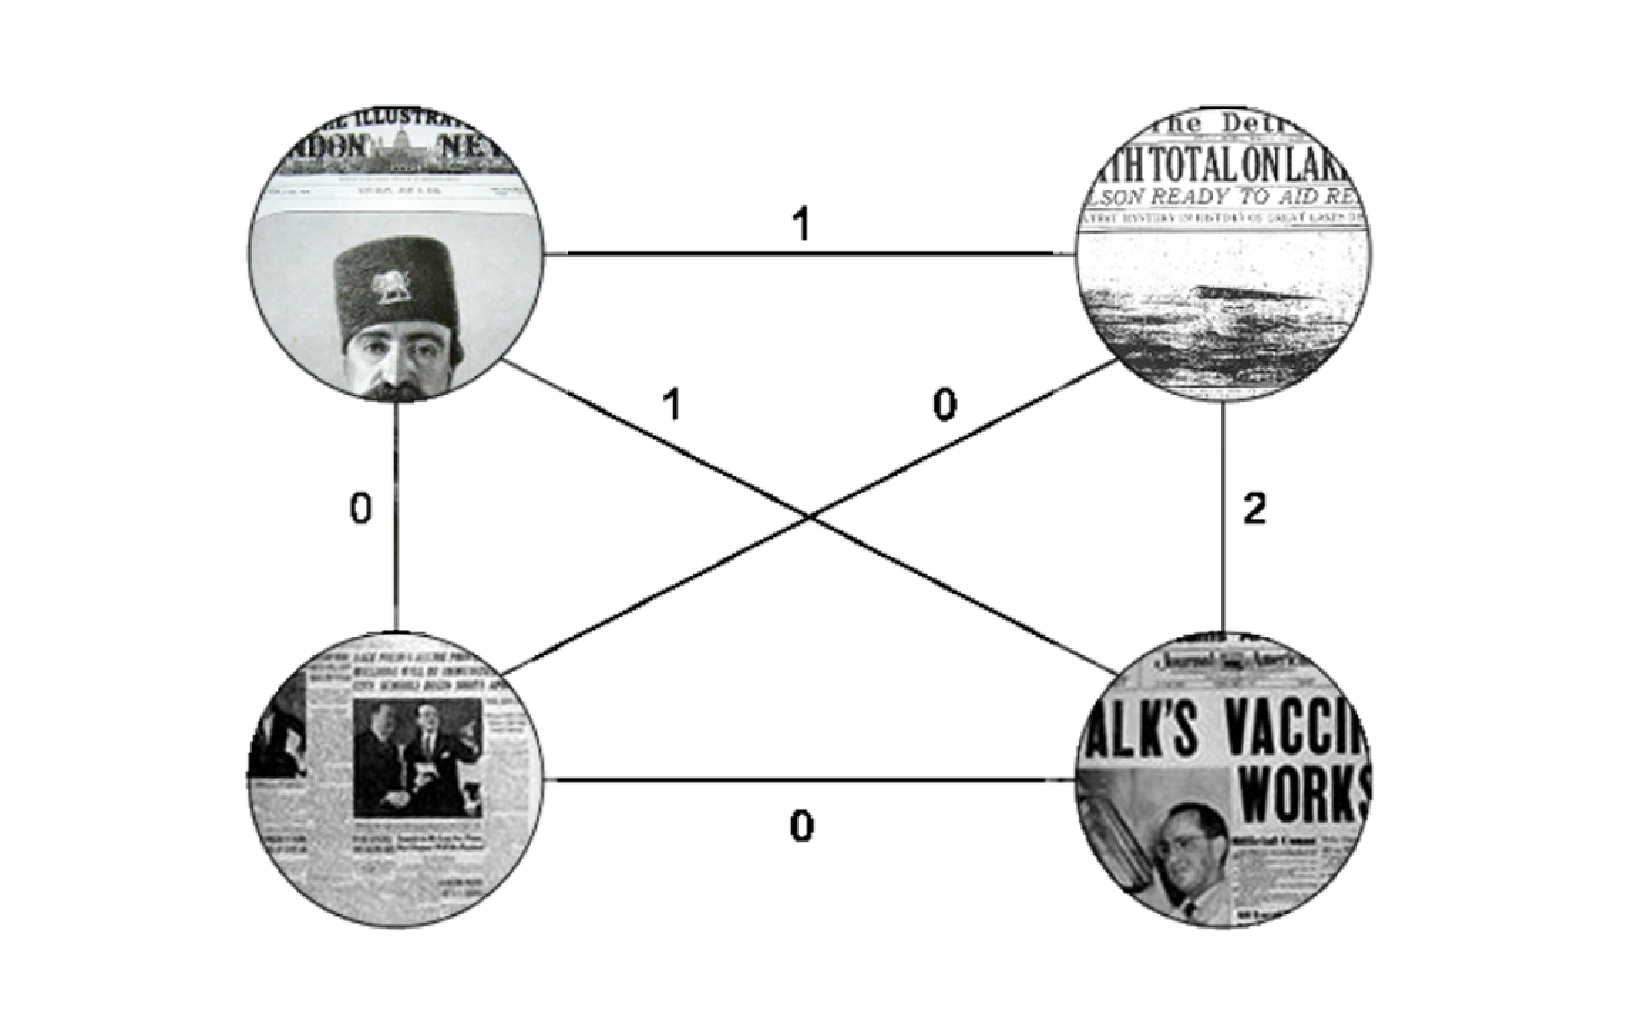
\includegraphics[width = 400pt]{verkkouusitaas.eps}\caption{Uutisartikkelit verkkona, jossa painoina kanssavierailujen lukumäärät.}
\label{verkko}
\end{figure} 

Covisitation("kanssavierailu") esiteltiin projektin muistipohjaisena osiona. Kanssavierailu on tapahtuma, jossa sama käyttäjä klikkaa kahta artikkelia tietyn ajan sisällä. Voimme ajatella uutisartikkeleita kuvan \ref{verkko} tapaisena verkkona, jossa artikkelisolmut on painotettu kanssavierailujen lukumäärillä.   

Verkkoa käsitellään vierekkäisyyslistana, jonka avaimina on artikkeli-id:t.
Kun havaitaan käyttäjän $u_i$ klikkaavan artikkelia $s_k$, käydään läpi kyseisen käyttäjän klikkaushistoria $C_{u_{i}}$. Jokaisen artikkelin $s_k \in C_{u_{i}}$ kohdalla muokataan sekä $s_j$ ja $s_k$ vierekkäisyyslistoja lisäämällä niihin kyseiseen klikkaukseen viittaava uusi merkintä. Jos kyseiselle parille on jo olemassa merkintä, päivitetään verkon painoja siten, että vanhojen kanssavierailujen merkitys vähenee ajan mittaan.

Ryhmän tekemän evaluoinnin johtopäätöksenä todettiin näiden kolmen algoritmin tuottavan yhdessä hyviä suosittelutuloksia. Huomattavaa oli se, että suosittelusta on mahdollista tehdä skaalautuvaa ilman, että suosittelujen laatu heikkenee. Ryhmän kehittämä suosittelujärjestelmä ei ole sisältöriippuvainen, joten sen voi helposti sovittaa muillekin palveluille kuin Google Newsille~\cite{Das:2007:GNP:1242572.1242610}.

\section{Pohdinta}

Suosittelujärjestelmiä käytetään runsaasti kaikenlaisia tuotteita tarjoavissa palveluissa. Esimerkiksi kappaleessa 2.2 esitellyn Flickr-kuvapalvelun tunnisteiden suosittelussa tulee esille ikään kuin kahden kerroksen suosittelua. Ensimmäisellä kerroksella käyttäjille suositellaan tunnisteita, jotka sopivat heidän kuviinsa. Näitä hyviä tunnisteita käyttämällä mahdollistuu toinen suosittelukerros, eli kuvien suositteleminen niitä selaaville käyttäjille. Palvelu voi suositella käyttäjille heitä kiinnostavia kuvia käyttämällä joko sisältöpohjaista tai yhteistoiminnallista suosittelujärjestelmää, mutta emme perehtyneet tähän "ylempään kerrokseen"\ tarkemmin.

Kappaleessa 2.1 mainittiin tunnisteiden käytön olevan hyvä keino kerätä tietoa kuvan kaltaisista tuotteista, joista on muuten saatavissa vain vähän tietoa. Lisättäkööt kuitenkin, että on olemassa erilaisia tapoja analysoida kuvien sisältöä ilman tunnisteita~\cite{Sigurbjornsson:2008:FTR:1367497.1367542}. Voitaisiinkin ajatella olevan mahdollista perustaa tunnisteiden suosittelu näille tiedoille yhteisötiedon sijaan.

Sisältöpohjaiset suosittelujärjestelmät tuntuvat olevan sisällöstä annetun tiedon armoilla tuotteiden analysoinnissa. Esimerkiksi elokuvien kohdalla järjestelmä tietää suositeltavista tuotteista vain sen, mitä näistä on tekstimuodossa kirjoitettu~\cite{Ullman}. Jos tiedot ovat huonosti kuvaavia, järjestelmä ei sitä tiedä. 

Yhteistoiminnalliset järjestelmät sen sijaan perustavat tuotteiden suosittelun käyttäjien arvosteluille tuotteista, joten samaa ongelmaa ei ilmene. Tuotesuositus annetaan yksittäiselle käyttäjälle tämän kanssa samankaltaisten käyttäjien mieltymysten perusteella. Tämän vuoksi järjestelmä toimii parhaiten valtavirran mielipiteitä myötäilevien käyttäjien kohdalla~\cite{Burke:2002:HRS:586321.586352}. Vastaavasti voitaisiin kuvitella suosittelun olevan hankalaa, jos käyttäjä pitää aivan erilaisista tuotteista kuin valtaosa muista käyttäjistä.


Tutkielmassa tutustuttiin suosittelujärjestelmien kahteen yleisimmin käytössä olevaan tyyppiin eli sisältöpohjaisiin ja yhteistoiminnallisen suodattamisen järjestelmiin. Nämä eivät kuitenkaan ole ainoat olemassa olevat suosittelujärjestelmien tyypit. Muita muotoja on tietopohjaiset (knowledge-based), demografiset (demographic) ja hyötypohjaiset (utility-based) järjestelmät. Lisätietoa näistä löytyy Burken artikkelista~\cite{Burke:2002:HRS:586321.586352}. Tutkielman kannalta avoimeksi kysymykseksi jää, tuottaisiko myös näiden tyyppien yhdistelmät parempia tuloksia kuin mikään järjestelmätyyppi yksinään.

        
\section{Yhteenveto}

Suosittelujärjestelmiä käytetään muun muassa kuva- elokuva- ja uutisartikkelipalveluissa. Järjestelmät voidaan jakaa sisältöpohjaisiin tai yhteistoiminnallisen suodattamisen järjestelmiin sen perusteella, tarkastellaanko vain käyttäjän omaa osto-, arvostelu- tai selaushistoriaa vai myös muiden käyttäjien vastaavia historioita.

Sisältöpohjainen suosittelu perustuu yhden käyttäjän historiatietoihin ja tuotteiden vertailuun keskenään. Esimerkkinä sisältöpohjaisen suodattamisen suosittelujärjestelmästä esiteltiin hyödyllisten tunnisteiden suosittelu käyttäjille. Tunnisteita suositeltiin sen perusteella, miten usein tarkasteltavat tunnisteet esiintyivät yhdessä samoissa konteksteissa~\cite{Sigurbjornsson:2008:FTR:1367497.1367542}.
 
Yhteistoiminnalliseen suodattamiseen perustuvassa suosittelussa keskitytään käyttäjäyhteisön välisiin relaatioihin. Samoja tuotteita kuluttaneiden käyttäjien oletetaan pitävän myös sellaisista tuotteista, joita vain toinen heistä on kuluttanut. Tutkielmassa esitelty elokuvien suosittelujärjestelmä käytti kahta yhteistoiminnallisen suodattamisen yleisintä mallia~\cite{Koren:2008:FMN:1401890.1401944}. Myös Google News -palvelulle kehitetty uutisartikkelien suosittelujärjestelmä käytti useamman mallin yhdistelmää. Muistipohjaisena algoritmina toimi kanssavierailu (covisitation) ja mallipohjaisina PLSI ja MinHash~\cite{Das:2007:GNP:1242572.1242610}.

Sisältöpohjaisen ja yhteistoiminnallisen suosittelujärjestelmän ero on pohjimmiltaan siinä, käytetäänkö suositteluun vain yhden käyttäjän vai koko käyttäjäyhteisön mieltymyksiä. Tehokkaimmat tulokset näytettäisiin saavan käyttämällä useamman kuin yhden suosittelumallin yhdistelmää~\cite{Bell:2007:LNP:1345448.1345465}\cite{Burke:2002:HRS:586321.586352}\cite{Koren:2008:FMN:1401890.1401944}.





% -akoskdoasjfoasf-- References ---
%
% bibtex is used to generate the bibliography. The babplain style
% will generate numeric references (e.g. [1]) appropriate for theoretical
% computer science. If you need alphanumeric references (e.g [Tur90]), use
%
% \bibliographystyle{babalpha-lf}
%
% instead.

\bibliographystyle{babplain-lf}
\bibliography{references-fi}


% --- Appendices ---

% uncomment the following

% \newpage
% \appendix
 
% \section{esimerkki}

\end{document}
